\documentclass[12pt]{article}

%% ── Packages ──────────────────────────────────────────────────────────────
\usepackage[margin=1in]{geometry}
\usepackage{setspace}
\usepackage{booktabs}
\usepackage{tabularx}
\usepackage{graphicx}
\usepackage{float}
\usepackage{amsmath}
\usepackage{amssymb}
\usepackage{natbib}
\usepackage{hyperref}
\usepackage{authblk}
\usepackage{abstract}
\usepackage{titlesec}
\usepackage{microtype}
\usepackage{mathptmx}
\usepackage[T1]{fontenc}
\usepackage[utf8]{inputenc}
\usepackage{caption}
\usepackage{subcaption}
\usepackage{rotating}
\usepackage{pdflscape}
\usepackage{xcolor}
\usepackage{enumitem}
\usepackage{footmisc}
\usepackage{nicefrac}
\usepackage{endnotes}

%% ── Hyperref setup ────────────────────────────────────────────────────────
\hypersetup{
  colorlinks=true,
  linkcolor=black,
  citecolor=black,
  urlcolor=black,
  pdftitle={When Does Political Competition Stabilize Growth? Evidence from Developing Democracies},
  pdfauthor={Bejar, Acosta y Lara, Moraes}
}

%% ── Section formatting ────────────────────────────────────────────────────
\titleformat{\section}{\normalfont\large\bfseries}{\thesection.}{0.5em}{}
\titleformat{\subsection}{\normalfont\normalsize\bfseries}{\thesubsection.}{0.5em}{}
\titlespacing*{\section}{0pt}{18pt}{8pt}
\titlespacing*{\subsection}{0pt}{12pt}{4pt}

%% ── Abstract formatting ───────────────────────────────────────────────────
\renewcommand{\abstractname}{\normalsize\bfseries Abstract}
\setlength{\absleftindent}{0.5in}
\setlength{\absrightindent}{0.5in}

%% ── Caption formatting ────────────────────────────────────────────────────
\captionsetup{font=small, labelfont=bf, margin=10pt}

%% ── Double spacing ────────────────────────────────────────────────────────
\doublespacing

%% ─────────────────────────────────────────────────────────────────────────
\begin{document}

%% ── Title block ───────────────────────────────────────────────────────────
\title{\large\bfseries When Does Political Competition Stabilize Growth?\\
Evidence from Developing Democracies\thanks{We thank participants at the Annual Meeting of the
Midwest Political Science Association and seminar participants at San Jos\'{e}
State University and Universidad de la Rep\'{u}blica for helpful comments.
All replication materials are available at
\url{https://github.com/Sergio-Bejar/growth\_LA}.}}

\author[1]{Sergio B\'{e}jar\thanks{Corresponding author: sergio.bejar@sjsu.edu}}
\author[2]{Federico Acosta y Lara}
\author[3]{Juan Andr\'{e}s Moraes}

\affil[1]{ Department of Political Science, San Jos\'{e} State University}
\affil[2]{ PhD Candidate, Department of Political Science, Washington University in St.\ Louis}
\affil[3]{ Department of Political Science, Universidad de la Rep\'{u}blica, Uruguay}

\date{\textit{Draft v6---please do not cite without authors' permission}}

\maketitle
\thispagestyle{empty}

%% ── Abstract ──────────────────────────────────────────────────────────────
\begin{abstract}
\singlespacing
\noindent Growth volatility is a central constraint on economic development:
it deepens poverty, shortens investment horizons, and destabilizes fragile
democracies. Yet developing countries with similar macroeconomic fundamentals
and exposure to external shocks often experience markedly different levels
of growth instability. We argue that a key but neglected source of this
variation is the structure of party competition. Investors in developing
democracies face two distinct sources of policy uncertainty: how much policy
will change across electoral outcomes, and how predictably a given
government will implement policy once in power. The first increases with
party system polarization; the second decreases. Their interaction produces
a U-shaped relationship between programmatic differentiation and growth
volatility. Using panel data from 16 Latin American democracies
(1994--2017), we find that both the linear and squared terms of Dalton's
party system polarization index are significant at the 1\% level, with a
turning point near 3.2 on a 0--10 scale. A mechanism investigation testing
nine candidate channels finds no sequential mediator; the effect operates
through a simultaneous shift in the aggregate expectations environment.
The pattern replicates in a global sample of 68 developing and developed
democracies before 2007 but attenuates afterward, consistent with a scope
condition: when large external shocks dominate, domestic political signals
lose their bite. These findings identify a political determinant of
growth volatility that operates within democratic regimes, complementing
existing work on macroeconomic fundamentals and institutional design.

\noindent\textit{Keywords:} growth volatility; party system polarization;
developing democracies; political economy of development; Latin America
\end{abstract}

\setcounter{page}{1}

%% ── Section 1: Introduction ───────────────────────────────────────────────
\section{Introduction}

A common assumption in both academic and policy circles is that ideological
moderation among political parties promotes macroeconomic stability.
Convergent party systems produce smaller policy shifts after elections,
which reduces uncertainty for investors and stabilizes growth. This
assumption is wrong. In developing democracies, the most volatile growth
environments are not those with the most polarized party systems. They are
those where parties are ideologically \textit{indistinct}. Moderate
polarization stabilizes growth. It is convergence, not polarization, that
is the underappreciated source of macroeconomic instability.

This matters because growth volatility is a central obstacle to economic
development: it deepens poverty, shortens investment horizons, and
destabilizes fragile democratic institutions \citep{Mobarak2005,
Loayza2007, HnatkovskaLoayza2005}. Democracies as a class mitigate
volatility relative to autocracies \citep{Knutsen2021,
MillemaciMonteforteTemple2025}, and the costs of failing to do so are
compounded when populist leadership erodes macroeconomic stability over
time \citep{FunkeSchularickTrebesch2023}. Yet developing countries with
similar macroeconomic fundamentals experience markedly different levels of
instability. Standard explanations \citep{Easterly2000, Ramey1995} leave
much of this variation unexplained, and the growth volatility literature
has almost entirely ignored how the structure of party competition shapes
investor expectations.

This paper argues that investors face two types of policy uncertainty, not
one. The first, how much policy will change across electoral outcomes,
increases with polarization. The second, how predictably a given government
will implement policy, \textit{decreases} with it. Their interaction
produces a U-shaped relationship between party system polarization and
growth volatility. We formalize this through a variance decomposition of
total policy uncertainty in Section~2.

Figure~\ref{fig:vol_la} documents the variation in growth volatility across
Latin America. Figure~\ref{fig:pol_la} plots polarization against growth
volatility: the binned conditional means trace the predicted U-shape, with
a minimum near our estimated turning point of $P^* = 3.21$.

\begin{figure}[H]
  \centering
  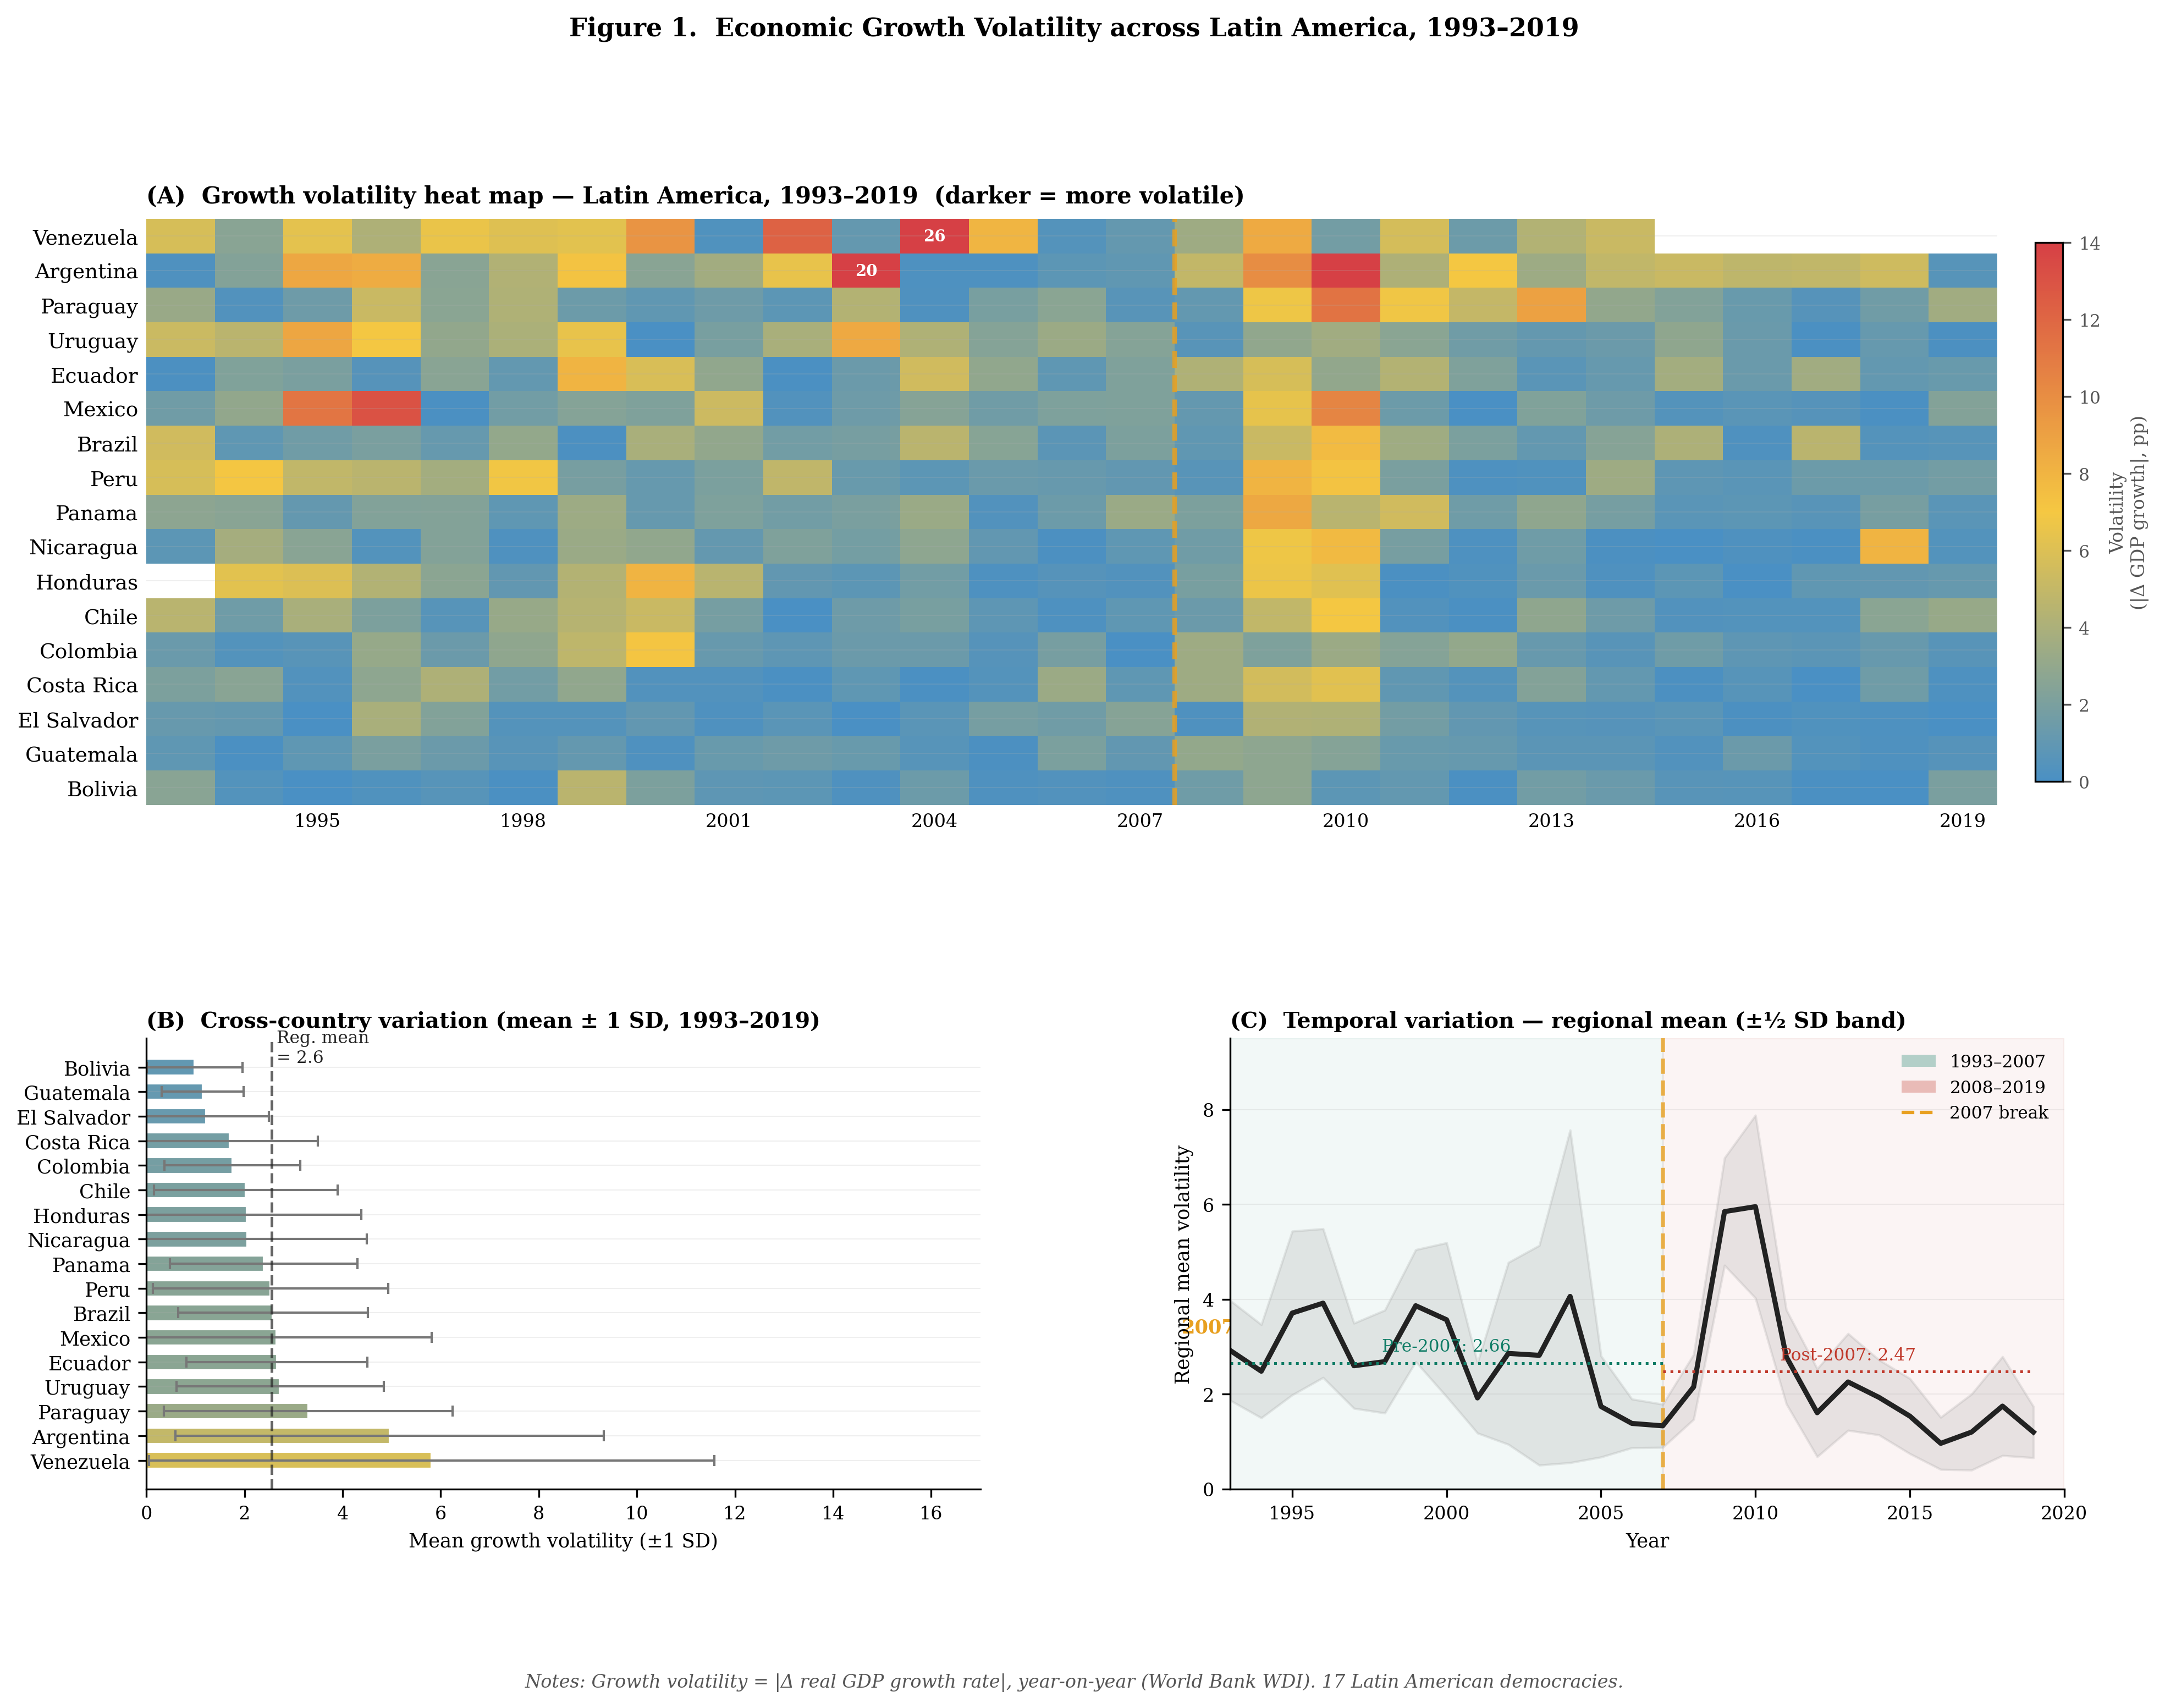
\includegraphics[width=\textwidth]{figures/fig1_volatility_LA.png}
  \caption{Variation in economic growth volatility across Latin America,
  1993--2019. Panel A shows a country $\times$ year heat map (darker cells =
  higher volatility). Panel B plots country-level means $\pm$1 SD, sorted
  by mean volatility. Panel C plots the regional annual mean with a
  $\pm$\nicefrac{1}{2} SD band, with the pre- and post-2007 period means
  indicated. Growth volatility = $|\Delta\text{real GDP growth rate}|$,
  year-on-year (World Bank WDI). 17 Latin American democracies.}
  \label{fig:vol_la}
\end{figure}

\begin{figure}[H]
  \centering
  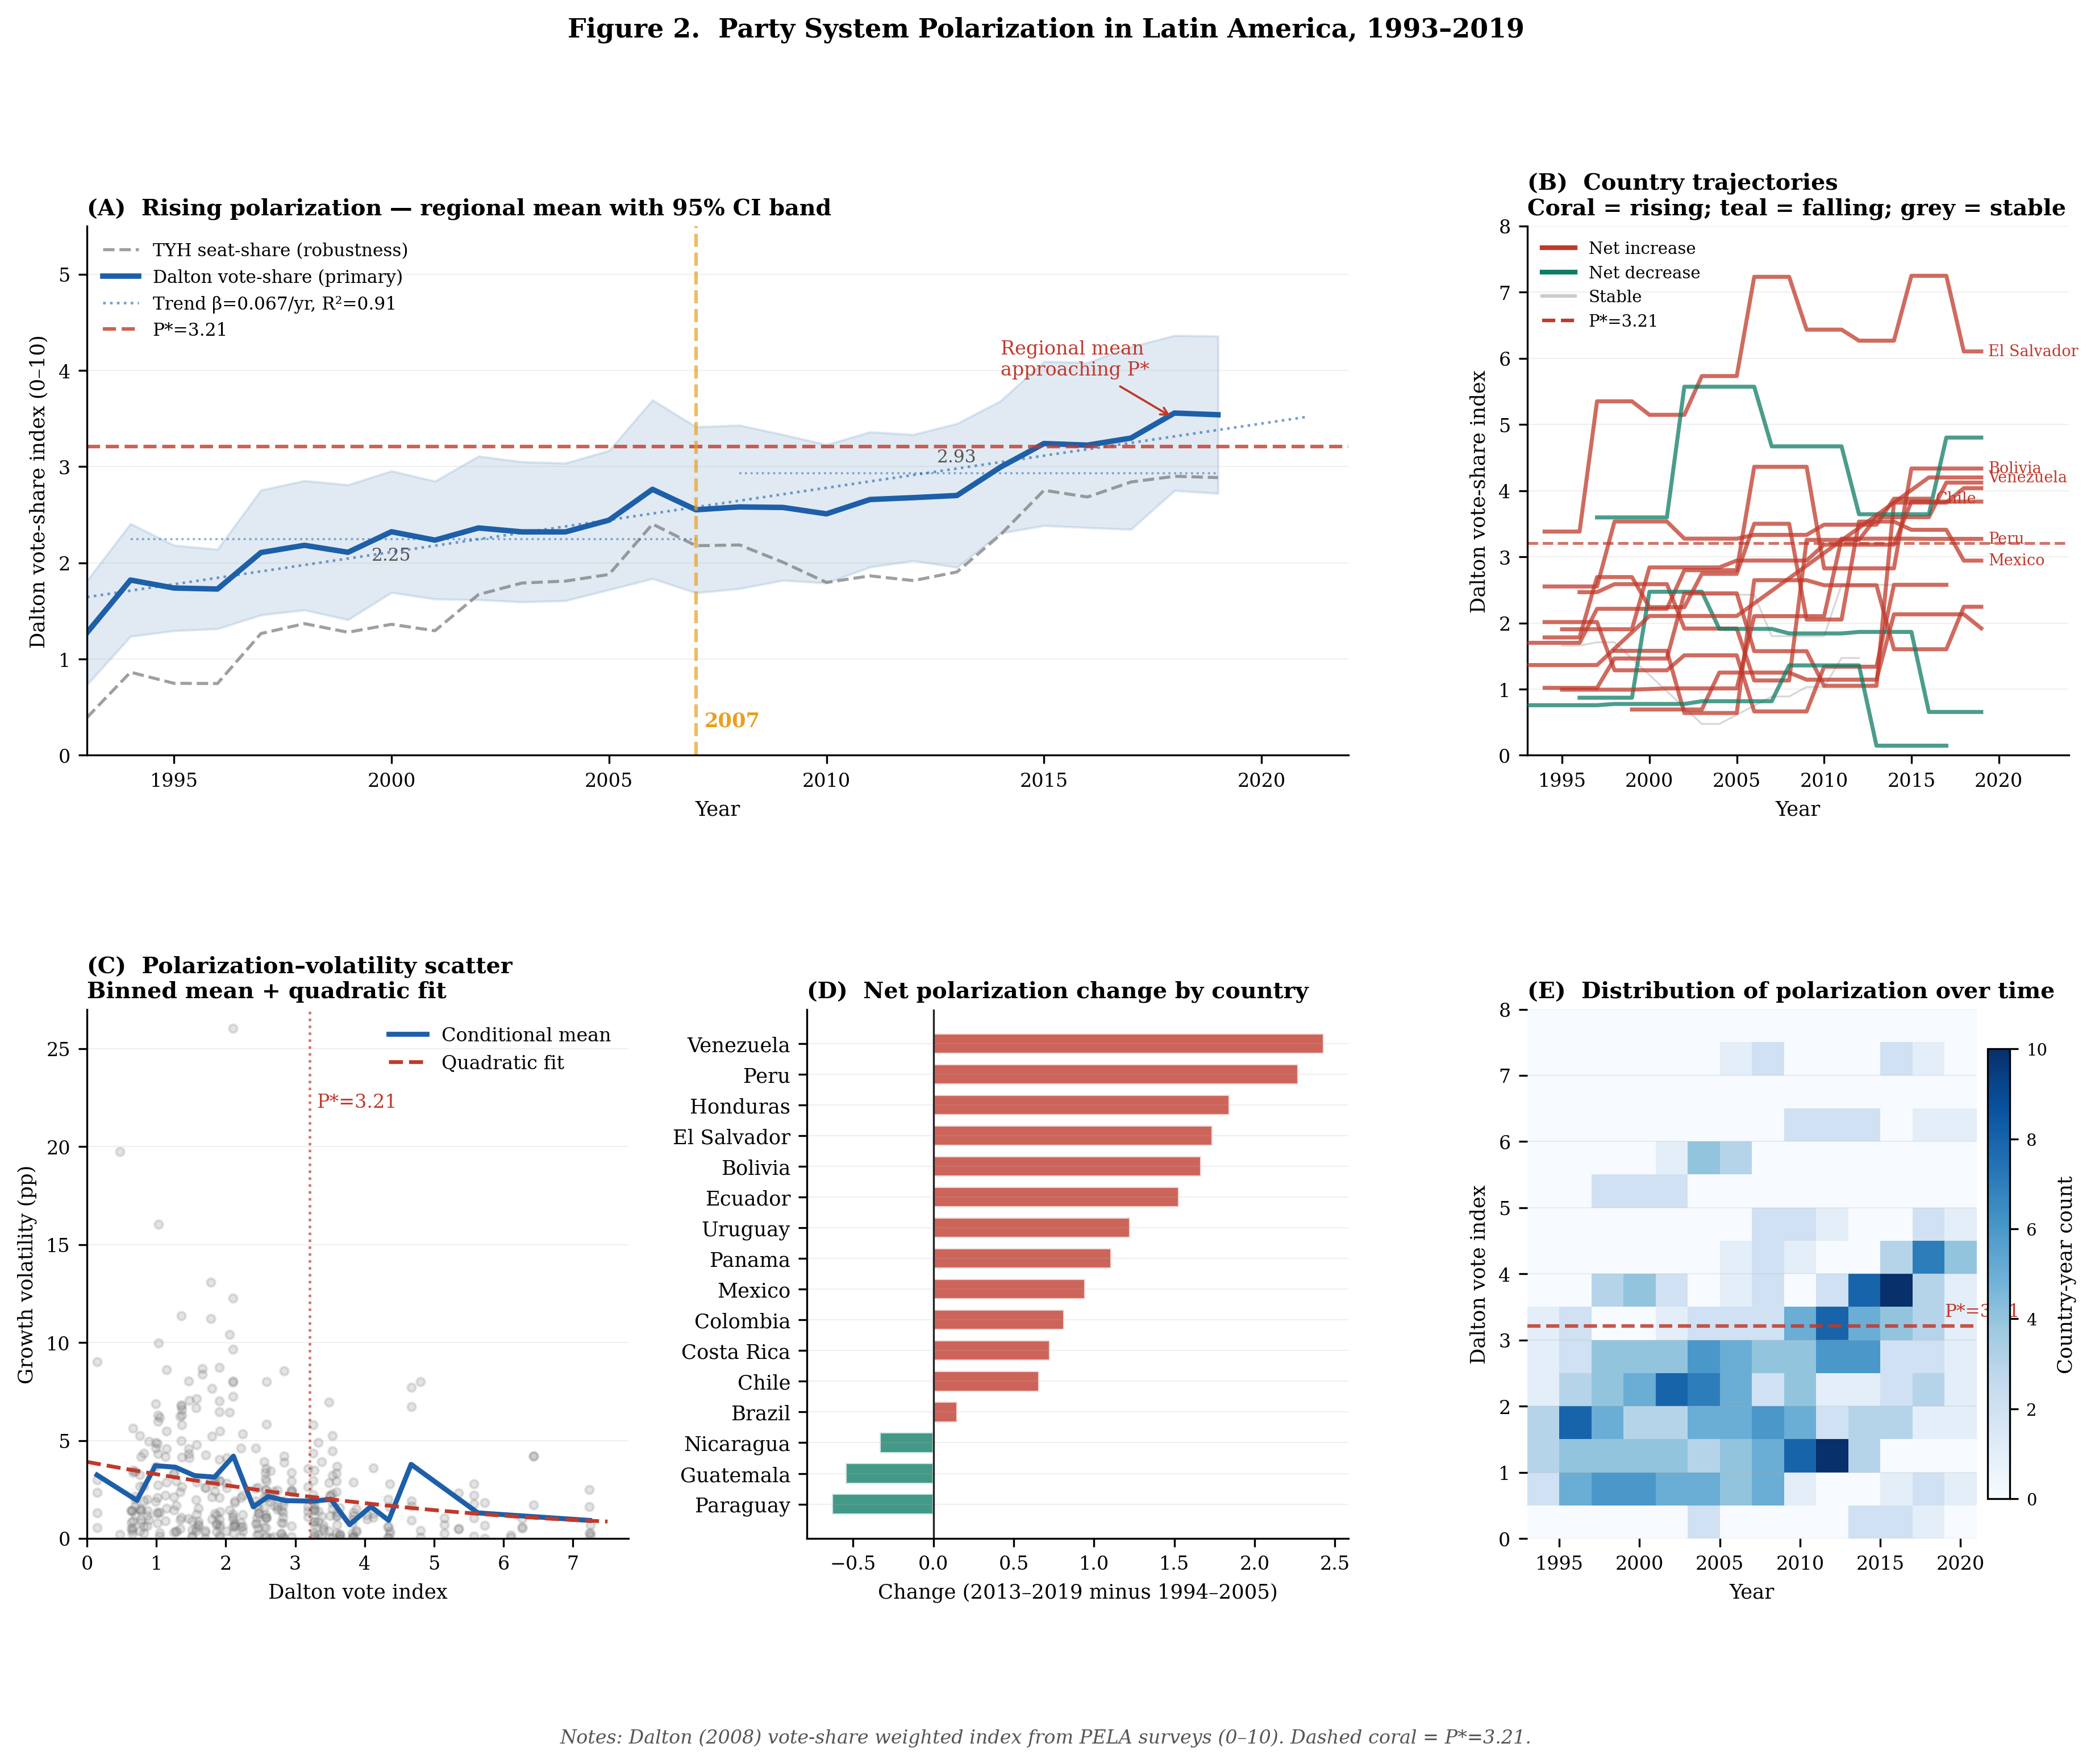
\includegraphics[width=\textwidth]{figures/fig2_polarization_LA.png}
  \caption{Party system polarization in Latin America, 1993--2019.
  Panel A: regional mean Dalton vote index with 95\% CI band and linear
  trend ($\beta = 0.067$/yr, $R^2 = 0.91$). Dashed coral line = estimated
  turning point $P^* = 3.21$.
  Panel B: country-level trajectories (coral = net increase $>0.3$;
  teal = net decrease).
  Panel C: raw scatter of polarization against growth volatility with
  binned conditional mean (blue) and quadratic fit (dashed coral).
  Panel D: net change by country (late 2013--2019 minus early 1994--2005).
  Panel E: distribution of country-years across polarization levels over
  time. Polarization = Dalton (2008) vote-share weighted index (PELA surveys).}
  \label{fig:pol_la}
\end{figure}

Using Dalton's \citeyearpar{Dalton2008} vote-share weighted polarization
index from elite legislative surveys (PELA), we estimate two-way fixed
effects models in a panel of 16 Latin American developing democracies from
1994 to 2017. Both the linear and squared terms are significant at the 1\%
level. The turning point lies near 3.2 on a 0--10 scale, at the 75th
percentile of observed polarization, meaning most country-years sit on the
downward arm of the U where more polarization is associated with less
volatility. Lagged specifications support a polarization-to-volatility
direction. A global extension recovers the U-shape in 68 democracies before
2007. Nine candidate mechanisms produce null sequential mediation results;
the effect operates through a simultaneous shift in the aggregate
expectations environment. The relationship attenuates after 2007, consistent
with a scope condition: when large external shocks dominate, domestic
political signals lose their bite.

This paper contributes to the development literature in three ways. First,
it identifies a political determinant of growth volatility that operates
\textit{within} democratic regimes, complementing existing work on
macroeconomic fundamentals and regime type \citep{Knutsen2021,
Mathonnat2018}. Second, it shows that the effect
of political competition on stability is nonlinear, overturning the
conventional expectation that polarization uniformly increases volatility.
Third, it identifies scope conditions under which political structures
matter most, particularly in periods not dominated by large external shocks.

The paper proceeds as follows. Section~2 develops the theoretical framework.
Section~3 describes the data and estimation strategy. Section~4 presents the
main results. Section~5 examines robustness. Section~6 investigates
mechanisms. Section~7 extends the analysis globally. Section~8 discusses
development implications. Section~9 concludes.


\section{Theoretical Framework}

The existing literature on polarization and economic performance predicts a
monotone positive relationship between polarization and growth volatility:
as parties diverge, the expected magnitude of policy change following
elections increases, investors discount long-term commitments, and volatility
rises \citep{Frye2002, AzzimontTalbert2014, Scartascini2013}. Recent
cross-national evidence confirms the negative linear relationship:
\citet{DornFuestImmelNeumeier2025} find that polarization reduces growth
through lower private investment, human capital investment, and total factor
productivity in a panel of 75 countries, and \citet{Azzimonti2018} shows
that partisan conflict depresses private investment in the United States.
\citet{BakerBloomDavisRodden2020} show that polarized elections generate
spikes in economic policy uncertainty, with downstream effects on firm
behavior. \citet{CarnahanSaiegh2020} document that unpredictable, decisive
elections in Latin American two-round systems increase stock market
volatility by roughly 80\%, and a growing body of evidence confirms that
partisan divisions now shape financial decisions across households,
corporate executives, and intermediaries \citep{KempfTsoutsoura2024}. This
argument is intuitive and supported by growing evidence, but it captures
only one of the two channels through which polarization affects investor
uncertainty.

The missing channel concerns what the conventional argument holds constant.
The standard framework focuses on the \textit{between-regime} component of
policy uncertainty, how much policy will differ depending on which party
wins, but treats as fixed the \textit{within-regime} component: how uncertain
investors are about what a given party will actually do once in power. This
paper builds on the existing framework by showing that within-regime
uncertainty is itself a function of polarization, and that the two
components move in opposite directions. Their interaction produces a
nonlinear total effect on investor uncertainty. We develop this argument
formally below.

\subsection{The Investor's Problem: Policy Uncertainty as a Variance
Decomposition}

Consider an investor allocating capital across periods in a democratic
political economy. The investor's problem is to forecast the policy
environment $\tilde{p}$ (a vector including tax rates, regulatory
intensity, trade policy, and property rights protection) over the relevant
investment horizon. The realized policy environment depends on electoral
outcomes that are uncertain at the time of investment. Formally, let $e \in
\{L, R\}$ denote the electoral outcome, realized with probabilities
$\Pr(e = R) = \pi$ and $\Pr(e = L) = 1 - \pi$, where $\pi$ reflects the
electoral competitiveness of the contest. Conditional on the electoral
outcome, the investor forms beliefs about realized policy: $\tilde{p} \mid
(e = j) \sim F_j(\mu_j, \sigma_j^2)$ for $j \in \{L, R\}$, where $\mu_j$
is the expected policy under party $j$ and $\sigma_j^2$ is the conditional
variance around that expectation.

The quantity that enters the investor's decision is the \textit{total
variance} of the policy environment:
\begin{equation}
\label{eq:decomp}
\textstyle\text{Var}[\tilde{p}] = \underbrace{\pi(1-\pi)(\mu_R - \mu_L)^2}_{V_B:
\text{ between-regime variance}} + \underbrace{\pi\sigma_R^2 +
(1-\pi)\sigma_L^2}_{V_W: \text{ within-regime variance}}
\end{equation}

\noindent This is the standard law of total variance applied to the mixture
distribution of policies.\footnote{The decomposition follows from
$\text{Var}[\tilde{p}] = \mathbb{E}[\text{Var}[\tilde{p}\mid e]] +
\text{Var}[\mathbb{E}[\tilde{p}\mid e]]$, which yields equation
(\ref{eq:decomp}) for a binary electoral outcome. The decomposition
generalizes to multi-party systems with multiple electoral scenarios, with
$V_B$ representing the variance of expected policies across scenarios weighted
by their probabilities.} The between-regime component $V_B$ captures the
standard policy risk argument: it increases in the squared ideological
distance $(\mu_R - \mu_L)^2$ between the competing parties. The within-regime
component $V_W$ captures something the conventional argument ignores: even
knowing who wins, how predictable is policy? A party that wins the election
may still govern in ways that deviate substantially from its stated positions
, whether opportunistically or because coalition bargaining, institutional
constraints, or interest-group pressure pull realized policy away from the
electoral platform.

The conventional argument, in our framework, analyzes only $V_B$ and assumes
$V_W$ is constant. We argue that this assumption fails systematically:
$V_W$ is itself a decreasing function of party system polarization. The
nonlinearity in total policy uncertainty follows as a consequence.

\subsection{Polarization and the Two Components of Policy Uncertainty}

\paragraph{Between-regime variance.} Let party system polarization $P$
be proportional to the ideological distance between the parties:
$P \propto |\mu_R - \mu_L|$.\footnote{This proportionality holds under
Dalton's \citeyearpar{Dalton2008} index, which calculates the
vote-share weighted standard deviation of party positions. The specific
formula is $PI = \sqrt{\sum_i p_i [(\bar{x}_i - \bar{x})/5]^2}$, which
is increasing in pairwise ideological distances weighted by electoral
relevance.} Then $V_B = \pi(1-\pi)P^2$ is \textit{increasing and convex}
in $P$. This is the conventional result: as parties diverge, the
spread of possible policy environments widens quadratically. The marginal
contribution of additional polarization to between-regime variance is
$\partial V_B / \partial P = 2\pi(1-\pi)P$, which is increasing in $P$.
The between-regime channel, taken alone, always argues for less polarization.

\paragraph{Within-regime variance.} The within-regime component $V_W$
is determined by how predictable each party is as a governing agent, which
we argue is \textit{decreasing in polarization}. The mechanism has three
reinforcing channels.

\textit{Reputational costs of deviation.} As parties occupy distinctive
ideological positions, their electoral constituency becomes more concentrated
and ideologically defined. Deviation from the platform imposes larger
reputational costs because the party's core voters, precisely those who
chose it for its ideological identity, are the most sensitive to betrayal
\citep{PerssTabellini2000}. \citet{Keefer2007} shows that young democracies
with non-programmatic parties cannot make credible policy commitments,
leading to short-termist and clientelistic governance.
\citet{BolWilliamson2019} document the costs of this unpredictability
directly: countries experiencing volatile institutional reform paths
suffer lower growth rates, with a one-standard-deviation increase in
institutional volatility reducing growth by approximately 0.5 percentage
points. A centrist party
that promises vague moderation can implement almost any policy without
alienating its median-voter base.
A clearly left-wing party that nationalizes industries deviates only mildly
from its supporters' expectations; a clearly left-wing party that privatizes
massively faces a catastrophic credibility loss. Higher polarization
therefore increases the cost of within-regime policy surprises, tightening
the distribution of realized policy around the electoral platform.

\textit{Organizational consistency.} Party systems with high programmatic
differentiation produce parties with stronger internal discipline and more
developed organizational infrastructure \citep{MainwaringScully1995,
KitscheltKselman2013}. Party
organizations built around ideological commitments generate consistent policy
signals over time, selecting candidates with coherent platforms, building
bureaucratic capacity around specific policy areas, and socializing members
into shared policy frameworks. These organizational features reduce the
variance of realized policy independently of any given election's outcome.
\citet{Mainwaring1995} documents precisely this pattern in Latin American
party systems: institutionalized, programmatically differentiated parties
deliver more consistent governance than clientelistic or personalistic ones,
regardless of their left-right position. \citet{RasmussenKnutsen2021}
extend this logic to policy outputs, showing that party
institutionalization is associated with more extensive and universal
welfare states, an effect that operates through precisely the
organizational consistency channel described here.

\textit{Investor learning.} When parties have clear and stable ideological
identities, investors can update their beliefs about post-election policy
more efficiently. Repeated interaction with a predictably left-wing or
predictably right-wing party reduces Bayesian uncertainty about its
policy intentions. \citet{LupuRiedl2013} argue that political uncertainty
in developing democracies is shaped precisely by the degree to which
party systems provide stable, identifiable alternatives.
\citet{Baker2016} show that policy uncertainty (as
measured by their EPU index) is substantially higher when the
composition of government is ideologically ambiguous. Recent evidence
confirms that polarization shapes economic expectations directly:
\citet{Guirola2025} finds that party polarization accounts for 57\% of
the variation in partisan differences in economic expectations across 27
European countries, though \citet{MianSufiKhoshkhou2023} caution that
partisan expectation gaps do not always translate into changes in actual
household spending. Our argument implies that the party system is an
upstream determinant of the EPU: higher programmatic differentiation at
the party system level reduces the residual uncertainty that the EPU
captures.

Formalizing these three channels: let $\sigma_j^2(P)$ denote
the within-regime variance of party $j$'s policy as a function of system
polarization. We assume $\partial \sigma_j^2 / \partial P < 0$, with
$\partial^2 \sigma_j^2 / \partial P^2 > 0$: within-regime variance is
decreasing in polarization but at a diminishing rate, as programmatic
clarity reaches a floor beyond which additional polarization cannot further
reduce policy variance.\footnote{This follows naturally from the reputational
cost argument: the marginal reduction in deviation risk from additional
ideological differentiation diminishes as the party is already well-defined.
Formally, $\sigma_j^2(P)$ can be modeled as a convex decreasing function such
as $\sigma_j^2 = \bar{\sigma}^2 e^{-\alpha P}$ for some $\alpha > 0$, though
the qualitative results do not depend on this functional form.} The
within-regime component of total policy uncertainty therefore satisfies
$\partial V_W / \partial P < 0$ and $\partial^2 V_W / \partial P^2 > 0$.

\paragraph{The turning point.} Total policy uncertainty is:
\begin{equation}
\label{eq:total}
\text{Var}[\tilde{p}](P) = \underbrace{\pi(1-\pi)P^2}_{V_B(P)} +
\underbrace{\pi\sigma_R^2(P) + (1-\pi)\sigma_L^2(P)}_{V_W(P)}
\end{equation}

\noindent where $V_B$ is increasing and convex in $P$, and $V_W$ is
decreasing and convex in $P$. At low polarization, $V_B \approx 0$ and
$V_W$ is large; total uncertainty is high and dominated by within-regime
unpredictability. As $P$ increases from zero, $V_B$ grows quadratically
from near zero while $V_W$ falls, and $\partial V_W / \partial P$ is
initially large in magnitude. For small $P$, the rate of decrease of
$V_W$ exceeds the rate of increase of $V_B$, so total variance falls.

The turning point $P^*$ is defined by:
\begin{equation}
\label{eq:turning}
\left.\frac{\partial \text{Var}[\tilde{p}]}{\partial P}\right|_{P=P^*} = 0
\quad\Longleftrightarrow\quad
2\pi(1-\pi)P^* = -\frac{\partial V_W}{\partial P}\bigg|_{P=P^*}
\end{equation}

\noindent At $P^*$, the marginal increase in between-regime variance exactly
equals the marginal decrease in within-regime variance. Below $P^*$, total
uncertainty falls with polarization; above $P^*$, it rises. This is the
turning point of the U-shape, derived from the structure of the theory and
not from the data. Our empirical estimate of $P^* \approx 3.2$ on the
Dalton 0--10 scale quantifies this threshold in the Latin American
institutional context.

Proposition 1 formalizes:

\begin{quote}
\textbf{Proposition 1.} Under the conditions described above, total policy
uncertainty $\text{Var}[\tilde{p}](P)$ is U-shaped in party system
polarization $P$. There exists a unique interior turning point $P^* \in
(0, P_{\max})$ below which total policy uncertainty is decreasing in $P$
and above which it is increasing in $P$.
\end{quote}

\noindent Since growth volatility is increasing in policy uncertainty
\citep{BejarMukherjee2011, Fatás2003, Baker2016, FernandezVillaverde2015},
Proposition 1 implies a
U-shaped relationship between party system polarization and growth volatility.
This is our primary prediction:

\begin{quote}
\textbf{Hypothesis 2 (H2):} \textit{The relationship between party system
polarization and growth volatility is curvilinear (U-shaped): growth
volatility first decreases as polarization increases from low to moderate
levels, then increases as polarization moves from moderate to high levels.}
\end{quote}

\noindent H2 subsumes the conventional linear argument as a special case:
over the upward arm of the U ($P > P^*$), the between-regime channel
dominates and more polarization generates more volatility, consistent with
\citet{Frye2002} and related work. The theoretical contribution is
identifying the downward arm, the region $P < P^*$ where the within-regime
clarity effect dominates, and explaining why previous scholarship has
missed it.

\paragraph{Why previous studies found linear effects.} Three features of
prior research produced linear estimates where the true relationship is
nonlinear. First, samples restricted to high-polarization contexts
\citep{Frye2002} observe only the upward arm of the U, where the between-regime
channel dominates. Second, polarization measures that conflate
between-regime distance with within-regime clarity (including aggregate
indices that assign high scores to both programmatically differentiated and
chaotically fragmented systems) suppress the within-regime variance
channel. The Dalton vote-share index, by measuring weighted ideological
distance among electorally relevant parties, captures the between-regime
component while correlating with the within-regime component through its
connection to party institutionalization. Third, the failure to separate
the two channels analytically meant that no existing framework predicted
a turning point, and linear specifications were imposed without theoretical
justification for doing so.

\subsection{Scope Conditions: When the Party System Signal Is Binding}

The decomposition in equation (\ref{eq:decomp}) assumes that the party system
is the primary source of policy uncertainty that investors face. This
assumption is plausible under conditions of relative external stability, when
the main source of uncertainty about the future policy environment is
domestic political competition. It fails when large external shocks dominate
investors' relevant information set.

\paragraph{External shocks and signal dominance.} When commodity price
booms, global financial crises, or sudden reversals in capital flows drive
macroeconomic outcomes, the party system signal is swamped. Investors'
relevant uncertainty is then about the external environment (commodity
prices, global interest rates, risk appetite), not about which domestic
party will win an election and what it will do. In Bayesian terms: the
prior over external states has such high variance that the party system
signal, even if highly informative about domestic policy, contributes
negligibly to the posterior over macroeconomic outcomes. The mechanism
through which polarization affects growth volatility is severed not because
party system structure no longer shapes policy signals, but because policy
signals no longer dominate the uncertainty that drives investment decisions
and growth volatility. Empirical evidence supports this structural break:
\citet{Aizenman2018} show that after 2008, growth in middle-income
countries became substantially more dependent on global factors (world
growth, oil prices, financial volatility) than on domestic institutional
variables. \citet{Abosedra2019} document that growth volatility spills
directionally from high-income to low-income countries, with transmission
lags of several years, and \citet{MumtazRuch2025} find that fiscal and
monetary policy uncertainty acts as a negative supply shock in 54
economies, explaining up to 12\% of output variation.

This reasoning generates a third hypothesis:

\begin{quote}
\textbf{Hypothesis 3 (H3):} \textit{The U-shaped relationship between party
system polarization and growth volatility attenuates when large external
shocks (commodity price cycles, global financial crises) dominate
domestic macroeconomic volatility.}
\end{quote}

\noindent H3 is independently motivated by \citet{Raddatz2007}, who
documents that external shocks are the primary driver of growth volatility in
developing economies during periods of commodity and financial turbulence,
and by \citet{FunkeST2016}, who show that financial crises generate
polarization endogenously, further obscuring the causal ordering from
party system structure to economic outcomes. The 2007--2008 global financial
crisis and the subsequent collapse and reversal of the commodity super-cycle
constitute the clearest instantiation of the conditions under which H3
predicts attenuation. The pre-2007 window provides the natural empirical
test of H1 and H2 in the absence of dominant external shocks.

\paragraph{Party institutionalization as a moderator.} A second scope
condition follows from the within-regime variance channel. Recall that
$\partial \sigma_j^2 / \partial P < 0$: polarization reduces within-regime
variance because clearer ideological positions generate reputational costs
for deviation. But this effect is stronger when parties are \textit{weakly}
institutionalized at baseline. Where party institutionalization is already
high, where parties have well-developed organizations, stable electoral
bases, and strong programmatic commitments regardless of polarization level,
the marginal benefit of additional polarization in reducing within-regime
variance is small, because within-regime variance is already low. The
turning point $P^*$ should therefore be \textit{lower} in countries with
more institutionalized party systems: less polarization is needed before
the between-regime channel begins to dominate.

This prediction is not directly testable in our data given the limited
within-country variation in party institutionalization, but it identifies
a heterogeneous treatment effect that future research can examine in
cross-national designs with larger samples.

\subsection{Auxiliary Implications: Domestic versus Foreign Investors}

The decomposition in equation (\ref{eq:decomp}) generates an additional
prediction about the \textit{differential} response of foreign and domestic
investors that is directly testable in our data.

Foreign direct investors face a distinctive version of the investment problem.
Unlike domestic investors, they operate across multiple country environments
and can reallocate capital internationally. Their primary concern is not
total policy uncertainty but the \textit{tail risk} of adverse policy
outcomes (nationalization, expropriation, discriminatory regulation)
that are concentrated in the high-polarization, left-winning scenario.
Because FDI involves long-horizon, relationship-specific capital that is
difficult to liquidate, foreign investors are particularly sensitive to the
between-regime variance channel: they weight heavily the scenario in which a
left-wing government dramatically shifts the regulatory environment.
\citet{KokashviliBarbakadze2020} find precisely this pattern: political
polarization is associated with reduced FDI inflows, with the effect
strongest where the left-wing electoral alternative has an explicitly
nationalist or redistributive agenda. The feedback loop is bidirectional:
\citet{CohleOrtega2022} show that FDI itself shifts vote shares toward
ideological extremes, suggesting that foreign capital flows and party
system polarization are jointly determined in developing democracies.

Domestic investors, by contrast, cannot relocate easily and must therefore
respond to \textit{total} policy uncertainty, both the between-regime
and within-regime components. Their investment decisions are sensitive to
the overall variance of the policy environment, not just to the downside
tail.

This differential response generates:

\begin{quote}
\textbf{Proposition 2.} The stabilizing effect of moderate polarization
on growth volatility operates primarily through the domestic investor
channel. FDI volatility should exhibit a different pattern, potentially
increasing with polarization over the range where domestic investor
stabilization occurs, because foreign investors respond primarily to
between-regime variance rather than total policy uncertainty.
\end{quote}

\noindent Proposition 2 explains what might otherwise appear as an
inconsistency in the mechanism analysis: the simultaneous observation of
decreasing growth volatility and increasing FDI volatility at moderate
polarization levels is not a failure of the theory but a prediction of it.
It implies that the growth stabilization documented in our main results
is driven by domestic investment behavior, a tightening of capital
allocation decisions by firms and households that face the improved
informational environment of moderate polarization, rather than by
foreign capital inflows.

\subsection{Hypotheses and Derivation Summary}

The theoretical framework generates three testable hypotheses and two
propositions. The first hypothesis reflects the conventional argument,
nested as a special case:

\begin{quote}
\textbf{Hypothesis 1 (H1):} \textit{Higher levels of party system
polarization increase growth volatility (the upward arm of the
U-shape, valid for $P > P^*$).}
\end{quote}

\noindent The primary prediction of the paper is:

\begin{quote}
\textbf{Hypothesis 2 (H2):} \textit{The relationship between party system
polarization and growth volatility is U-shaped. Growth volatility first
decreases as polarization increases from low to moderate levels (the
downward arm, valid for $P < P^*$), then increases as polarization moves
from moderate to high levels (the upward arm, valid for $P > P^*$). The
turning point $P^*$ is defined by equation (\ref{eq:turning}).}
\end{quote}

\noindent The scope condition is:

\begin{quote}
\textbf{Hypothesis 3 (H3):} \textit{The U-shaped relationship between
polarization and growth volatility attenuates in periods dominated by large
external shocks, when domestic political signals no longer constitute the
binding source of macroeconomic uncertainty.}
\end{quote}

\noindent Propositions 1 and 2 follow from the assumptions of the framework.
Proposition 1 establishes existence and uniqueness of the turning point $P^*$
under assumptions stated in subsection 2.2. Proposition 2 predicts divergence
between domestic and foreign investor responses over the stabilizing arm of
the U. Both propositions generate auxiliary implications that future research
can test, including the role of party institutionalization as a moderator of
$P^*$ (Proposition 1) and the domestic investment mechanism as the operative
channel (Proposition 2).

The theoretical framework, in sum, differs from the conventional argument not
by adding an additional linear channel but by respecifying the informational
problem investors face. It treats total policy uncertainty, not merely
between-regime distance, as the quantity that drives investment decisions
and growth volatility, and shows that the two components of total policy
uncertainty respond differently to party system polarization. The U-shape
follows from this respecification under plausible conditions, not as an
empirical observation seeking a theoretical home.


%% ── Section 3: Data and Methodology ─────────────────────────────────────
\section{Data and Methodology}

\subsection{Dependent Variable: Growth Volatility}

Our dependent variable is the absolute year-on-year change in the real GDP
growth rate:
\[
\text{Abs}(\Delta\text{growth})_{it} = |g_{it} - g_{it-1}|
\]
where $g_{it}$ is the real GDP growth rate for country $i$ at time $t$. This
measure accurately operationalizes temporal variance in growth within
countries \citep{BejarMukherjee2011, Mobarak2005, Denizer2002} and avoids
the biases of cross-sectional measures, which underestimate time-series
variance and are sensitive to outliers. Data are from the World Bank
Development Indicators (WDI). We use the natural logarithm of this measure
in all models to address right-skewness.

\subsection{Main Independent Variable: Party System Polarization}

Our primary polarization measure is Dalton's \citeyearpar{Dalton2008}
vote-share weighted ideological polarization index:
\[
\textstyle PI = \sqrt{\sum_{i=1}^{n} p_i \cdot \left(\frac{\bar{x}_i - \bar{x}}{5}\right)^2}
\]
where $p_i$ is the vote share of party $i$, $\bar{x}_i$ is its position on
the left-right scale, and $\bar{x}$ is the weighted mean across all parties.
The index ranges from 0 (complete convergence) to 10 (maximum dispersion).
We construct this index from the Programa de Elites Parlamentarias de
Am\'{e}rica Latina (PELA), which surveys legislators on their party's
left-right self-placement. The Dalton vote-share index correlates strongly
with the Taylor-Herman index ($r = .876$) and Huber's index ($r = .894$).
We also report results using Taylor-Herman seat-share and vote-share
alternatives as robustness checks.

\subsection{Sample and Controls}

Our primary Latin American sample comprises 16 democracies from 1994 to 2017,
restricted to country-years with a Polyarchy score $\geq 0.5$ on V-Dem for
which PELA data are available. The effective panel contains 292 country-year
observations. Controls follow the growth volatility literature
\citep{Easterly2000, BejarMukherjee2011, Mathonnat2018}: capital account
openness \citep{ChinnIto}, the liberal democracy index (V-Dem), log
inflation, government spending volatility, fixed capital formation volatility,
an election year dummy, mean district magnitude, and the effective number of
legislative parties \citep{Schmidt}. We include the lagged dependent variable
to account for temporal dependence in growth volatility.

Two measurement concerns deserve attention. First, the Dalton index is
constructed from PELA surveys of legislators, not from expert codings or
manifesto content analysis. Legislative self-placement introduces
measurement error: legislators may strategically misrepresent their party's
position, and small survey samples in some country-rounds raise concerns
about precision. Classical measurement error in the independent variable
would attenuate our estimates toward zero, making our significant results
conservative. Non-classical error (if legislators in volatile economies
systematically misreport positions) could introduce bias, though we are not
aware of evidence for this pattern in the PELA literature. Second, the
effective number of parties (ENP) and party system polarization are
conceptually related: fragmented systems can be either polarized or
convergent. Including both as regressors risks partial collinearity.
We retain ENP because it controls for the mechanical relationship between
fragmentation and volatility, but we note that our results survive
dropping ENP from the specification.

\subsection{Estimation and Identification}

Our baseline specification is:
\[
\log(\text{Abs}(\Delta g))_{it} = \alpha + \beta_1 \text{Pol}_{it} +
\beta_2 \text{Pol}^2_{it} + \boldsymbol{\gamma}\mathbf{X}_{it} +
\lambda_i + \delta_t + \varepsilon_{it}
\]
where $\lambda_i$ are country fixed effects and $\delta_t$ are year fixed
effects. A U-shaped relationship (H2) implies $\hat{\beta}_1 < 0$ and
$\hat{\beta}_2 > 0$, with turning point at $-\hat{\beta}_1 / (2\hat{\beta}_2)$.
We estimate all models using two-way fixed effects with standard errors
clustered at the country level.

\paragraph{Identification.} Country fixed effects absorb all time-invariant
confounders; year fixed effects absorb common time shocks. The primary
residual concern is contemporaneous reverse causality: volatile economies
may generate polarized party systems. We address this through three
strategies:

\begin{enumerate}[leftmargin=*, label=(\roman*)]
  \item \textit{Lagged specifications.} We estimate models at $t-1$ and
  $t-2$ lags of polarization. If reverse causality dominates, the
  contemporaneous specification should be strongest. We find that the
  $t-1$ specification recovers significance for the squared term while the
  $t-3$ lag fades, a pattern inconsistent with contemporaneous reverse
  causality and consistent with a 1--2 year institutional transmission lag.

  \item \textit{Period split.} We show that the relationship holds
  pre-2007 but attenuates post-2007. Since financial crises generate
  polarization endogenously \citep{FunkeST2016}, the pre-2007 window
  provides a cleaner identification environment. If the pre-2007
  finding were reverse-causal, the attenuation of the relationship
  in the more volatile post-2007 period should strengthen it, not weaken it.

  \item \textit{Out-of-sample replication.} We replicate the main
  finding in 62 non-Latin American democracies, ruling out
  unobserved regional confounders specific to Latin America as the
  driver of the relationship.
\end{enumerate}

This package does not achieve the causal identification of a natural
experiment or credible instrument. The reverse channel, from economic
outcomes to polarization, is itself empirically documented:
\citet{CohleOrtega2022} show that FDI inflows shift vote shares toward
ideological extremes, particularly benefiting right-wing parties, while
\citet{FunkeST2016} document that financial crises generate polarization
endogenously. These findings motivate our reliance on lagged specifications
and the pre-2007 period split. The evidence is consistent with the causal
interpretation but does not definitively establish it.

%% ── Section 4: Main Results ──────────────────────────────────────────────
\clearpage
\section{Main Results}

Figure~\ref{fig:main} presents the fitted partial-effect curves for our five
main specifications, with 95\% confidence intervals on the marginal effects.
The coefficient summary appears in Table~\ref{tab:main}.

\begin{figure}[H]
  \centering
  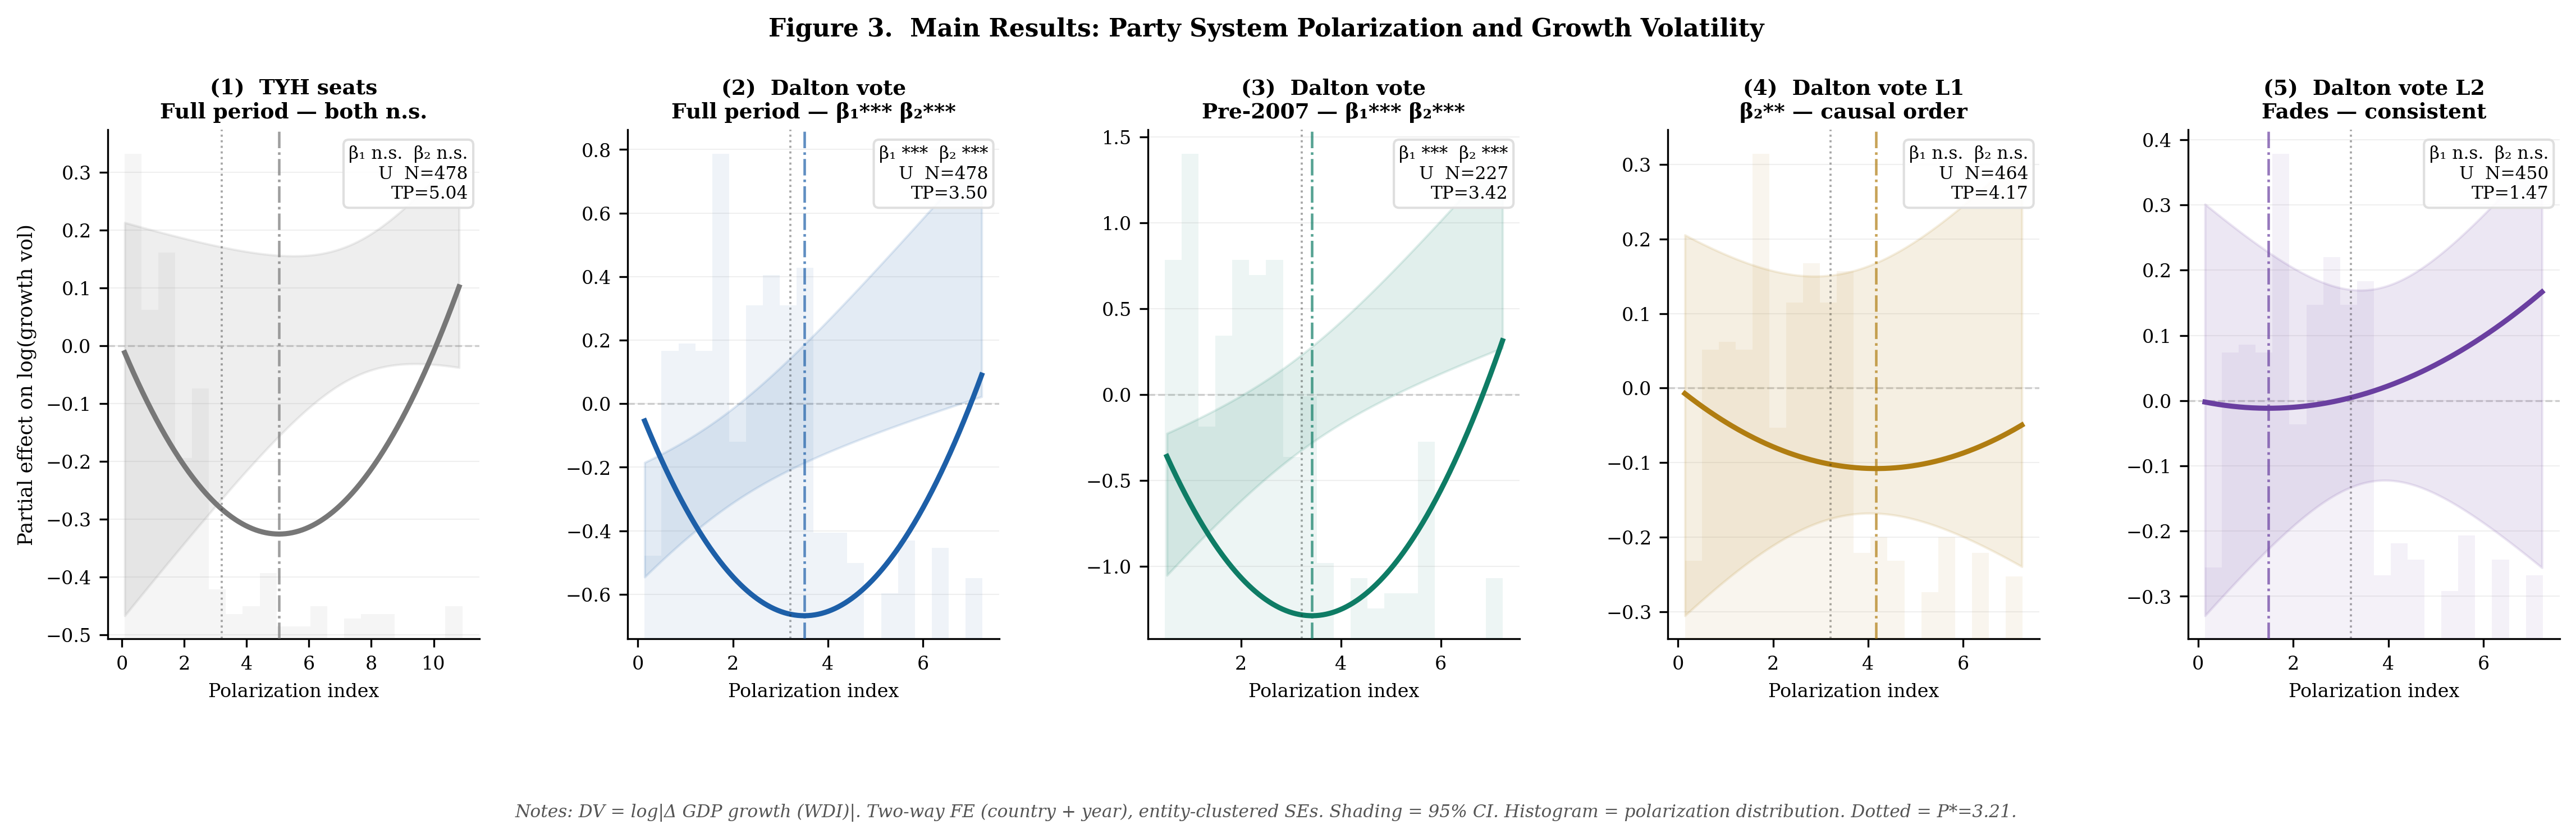
\includegraphics[width=\textwidth]{figures/fig_main.png}
  \caption{Fitted partial effects of party system polarization on log growth
  volatility across main specifications. Shading = 95\% CI on the marginal
  effect. Histogram = empirical distribution of polarization in the sample.
  DV = $\log|\Delta\text{GDP growth}|$. Two-way FE, entity-clustered SE.}
  \label{fig:main}
\end{figure}

\begin{table}[H]
\centering
\caption{Party System Polarization and Growth Volatility, Latin America}
\label{tab:main}

\begin{tabular}{@{}lp{1.8cm}p{1.8cm}p{1.8cm}p{1.8cm}p{1.8cm}@{}}
\toprule
 & (1) & (2) & (3) & (4) & (5) \\
 & TYH & Dalton & Dalton & Dalton & Dalton \\
 & 1994--2017 & 1994--2017 & pre-2007 & L1 lag & L2 lag \\
\midrule
Polarization ($\hat{\beta}_1$) & $-$0.181 & $-$0.660$^{***}$ & $-$0.893$^{***}$ & $-$0.313 & $-$0.019 \\
 & (0.213) & (0.135) & (0.255) & (0.196) & (0.142) \\[4pt]
Polarization$^2$ ($\hat{\beta}_2$) & 0.021 & 0.103$^{***}$ & 0.136$^{***}$ & 0.026$^{**}$ & 0.001 \\
 & (0.013) & (0.021) & (0.035) & (0.013) & (0.008) \\[4pt]
Lagged DV & 0.004 & 0.007 & $-$0.090$^{*}$ & 0.013 & 0.007 \\
 & (0.045) & (0.047) & (0.048) & (0.046) & (0.047) \\[4pt]
FCF volatility & 0.021$^{**}$ & 0.019$^{**}$ & 0.032$^{***}$ & 0.020$^{**}$ & 0.021$^{**}$ \\
 & (0.008) & (0.008) & (0.010) & (0.008) & (0.008) \\[4pt]
District magnitude & $-$0.006$^{***}$ & $-$0.006$^{***}$ & $-$0.002 & $-$0.006$^{***}$ & $-$0.006$^{***}$ \\
 & (0.002) & (0.002) & (0.004) & (0.002) & (0.002) \\[4pt]
Eff.\ N parties (ENP) & $-$0.121$^{*}$ & $-$0.109$^{*}$ & $-$0.318$^{***}$ & $-$0.123$^{*}$ & $-$0.110 \\
 & (0.062) & (0.064) & (0.115) & (0.063) & (0.068) \\
\midrule
Turning point & 4.27 & 3.21 & 3.28 & 6.01 & --- \\
Shape & U & U & U & U & --- \\
Controls & Yes & Yes & Yes & Yes & Yes \\
Country FE & Yes & Yes & Yes & Yes & Yes \\
Year FE & Yes & Yes & Yes & Yes & Yes \\
$N$ & 292 & 293 & 166 & 278 & 264 \\
$R^2$ (within) & 0.061 & 0.054 & 0.081 & 0.063 & 0.028 \\
\bottomrule
\multicolumn{6}{p{0.96\textwidth}}{\footnotesize\textit{Notes:} DV = $\log|\Delta\text{GDP growth (WDI)}|$. Controls include capital account openness, liberal democracy index, log inflation, spending volatility, FCF volatility, election year dummy, district magnitude, and effective number of legislative parties. Standard errors clustered at country level in parentheses. $^{***}p<0.01$; $^{**}p<0.05$; $^{*}p<0.10$.}
\end{tabular}
\end{table}

The results provide strong support for H2. Model (1) uses the
Taylor-Herman seat-share index; neither term achieves statistical
significance over the full period. Model (2) uses Dalton's vote-share
index, the measure directly motivated by PELA legislative surveys and the
paper's theoretical focus on programmatic differentiation. Both the linear
term ($\hat{\beta}_1 = -0.660$, $p < 0.01$) and squared term
($\hat{\beta}_2 = 0.103$, $p < 0.01$) are significant at the 1\% level,
with a turning point at 3.21 on the 0--10 scale. Model (3) restricts to the
pre-2007 period; both terms remain significant at 1\% with a stable turning
point at 3.28.

The measure matters. The Dalton vote-share index substantially outperforms
the seat-share alternative because it directly operationalizes what the
theoretical mechanism requires: the weighted ideological distance among
parties as voters, not legislatures, express it. Seat-share indices give
greater weight to small parties that win disproportionate legislative
representation under PR rules, potentially overstating the programmatic
content of their presence. Vote shares better capture the informational
environment investors observe.

Models (4) and (5) present lagged specifications. When polarization is
measured at $t-1$, the squared term is significant ($p < 0.05$); at $t-2$,
significance fades. This decay pattern is inconsistent with contemporaneous
reverse causality: were volatile economies generating polarized party systems,
we would observe a monotone decay from $t=0$ outward. Instead, the $t-1$
specification recovers significance relative to the contemporaneous baseline,
and then fades at $t-2$, a pattern consistent with a 1-year institutional
transmission lag from party system configuration to investor behavior to
macroeconomic outcomes.

Substantively, the turning point at 3.21 falls at approximately the 75th
percentile of the observed polarization distribution (mean = 2.6, 75th
percentile $\approx$ 3.4). Most Latin American country-years in our sample
therefore operate on the downward arm of the U, the region where more
polarization is associated with less volatility. The conventional linear
prediction that polarization monotonically increases volatility does not
describe the empirically dominant regime in the region.

%% ── Section 5: Robustness ─────────────────────────────────────────────────
\section{Robustness}

\subsection{Period Heterogeneity}

Split-sample results and the country-level decomposition of changes in
growth volatility across periods appear in Figure~\ref{fig:period} in the
Online Appendix.

In the pre-2007 Latin American sample, both the linear ($p < 0.10$) and
squared ($p < 0.05$) terms are significant. In the post-2007 sample, neither
term is significant. The post-2007 period scrambles the regional pattern in
ways orthogonal to domestic party systems. Uruguay and
Venezuela experience dramatic volatility reductions driven by commodity booms
and economic collapse respectively; Paraguay and Argentina become more
volatile for reasons unrelated to party system configuration. The polarization
signal cannot compete with these shocks.

The post-2007 attenuation is informative about causal direction. If volatile
economies were causing polarized party systems (reverse causality), the
relationship should strengthen in the more volatile post-2007 period, not
weaken. The opposite pattern supports the scope condition: the domestic
political channel operates when external stability allows party system
signals to bind.

\subsection{Lagged Specifications across Samples}

The lag structure across Latin American and global samples appears in
Figure~\ref{fig:lags} in the Online Appendix.
In the global pre-2007 sample, the squared term strengthens from $L0$
($p < 0.01$) to $L1$ ($p < 0.01$) to $L2$ ($p < 0.01$) before fading at
$L3$. In the Latin American sample, $L1$ recovers significance for the
squared term relative to the contemporaneous baseline before fading at $L2$.
Both patterns are inconsistent with contemporaneous reverse causality.

%% ── Section 6: Mechanism ──────────────────────────────────────────────────
\section{Mechanism Analysis}

Figure~\ref{fig:mech} presents the results of the mechanism investigation.

\begin{figure}[H]
  \centering
  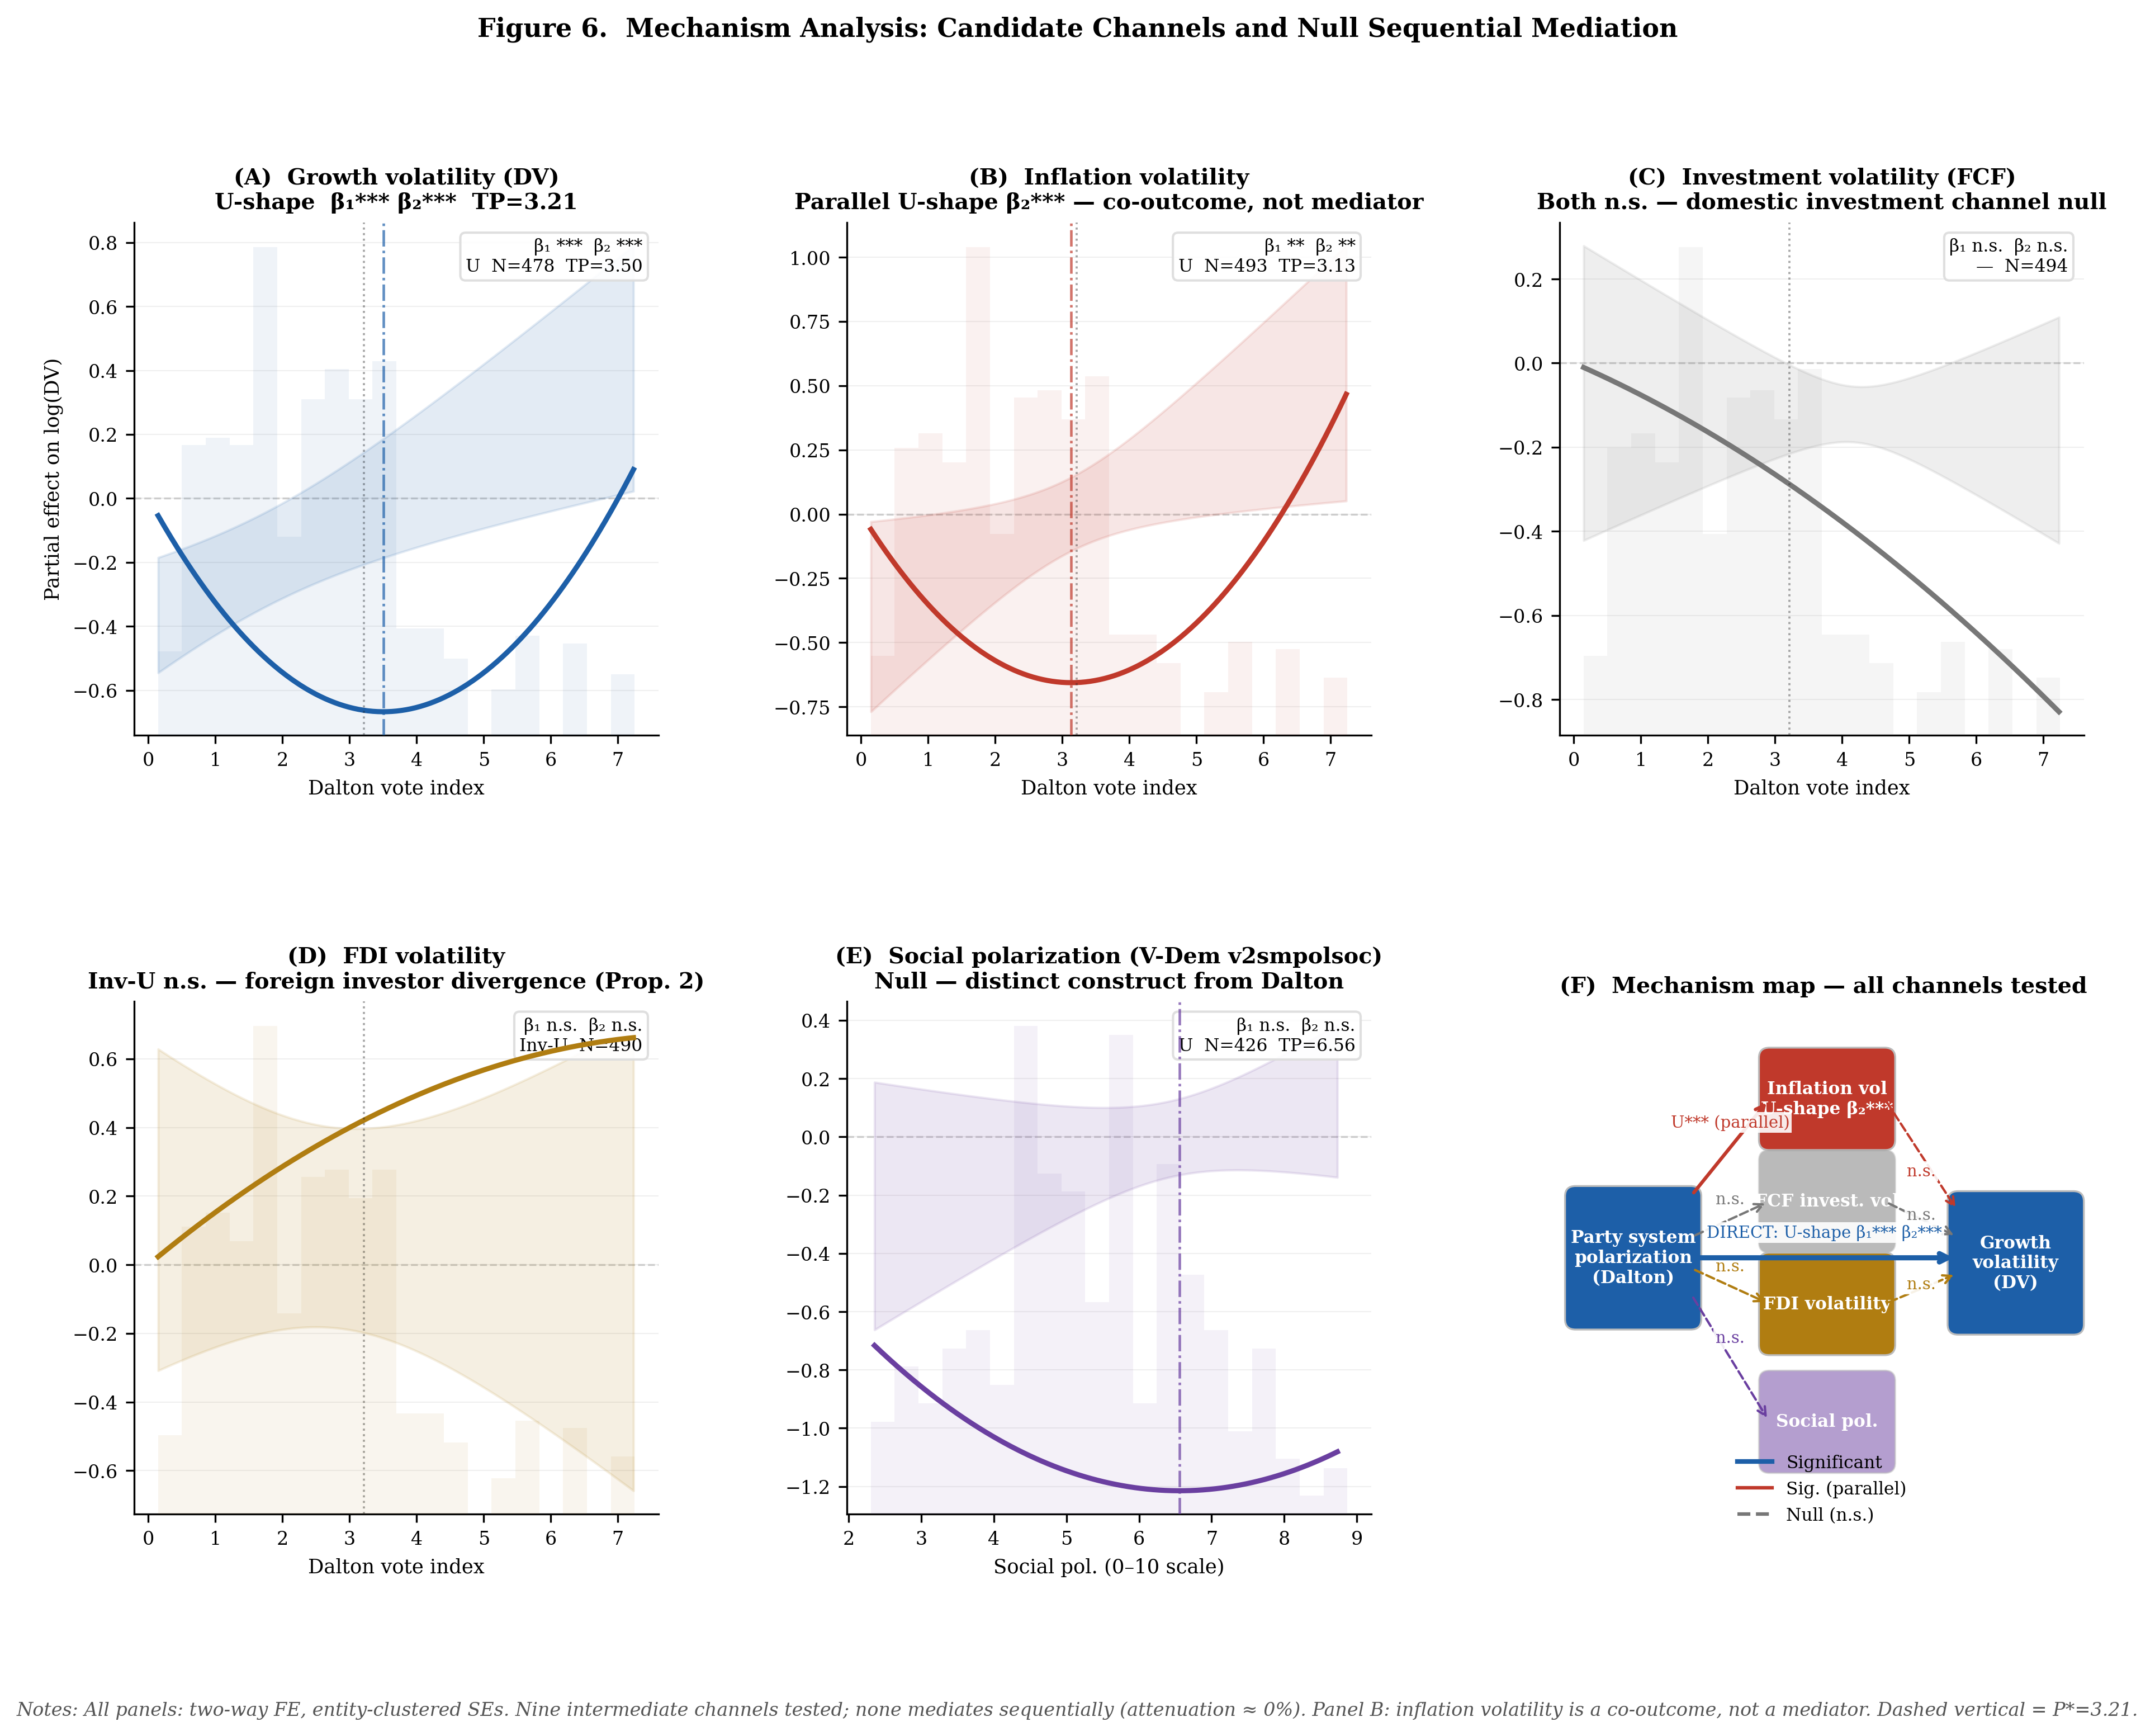
\includegraphics[width=\textwidth]{figures/fig_mechanism_full.png}
  \caption{Mechanism analysis. Panel A reproduces the main growth volatility
  result (U-shaped, Dalton vote). Panels B and C test the fiscal channel
  (spending volatility) and domestic investment channel (FCF volatility).
  Panel D tests the FDI volatility channel. Panel E shows the pre-2007
  mediation. Panel F presents the mechanism path diagram.}
  \label{fig:mech}
\end{figure}

We submit every credible annual intermediate variable to the same two-way
fixed effects specification used in the main analysis, testing whether it
(a) displays a quadratic relationship with polarization and (b) mediates
the polarization--volatility link sequentially. The candidate channels are:
domestic investment volatility (gross fixed capital formation), FDI
volatility, monetary volatility (M2 growth), trade openness volatility,
government spending volatility, inflation volatility, social polarization,
party institutionalization, and policy signal stability.

The results are uniformly null as sequential mediators. No intermediate
variable attenuates the direct effect of polarization on growth volatility
when included in the model. The fiscal channel, through which
\citet{BejarMukherjee2011} showed electoral system effects on spending
discretion produce growth volatility, does not operate here: polarization
does not predict spending volatility, and adding spending volatility as a
mediator produces zero attenuation of the polarization coefficients. This
null result is notable given \citet{Grechyna2021}'s finding that mandatory
spending can offset the macroeconomic volatility induced by polarization,
suggesting that the fiscal channel may operate only through specific
spending categories that our aggregate measure does not capture. The
domestic investment channel (FCF volatility) and monetary channel (M2) show
no quadratic relationship with polarization. Trade openness volatility is
similarly null.

The FDI channel produces a more nuanced but ultimately non-mediating
pattern. Polarization exhibits an inverted-U relationship with FDI
volatility ($\hat{\beta}_1 > 0$, $p < 0.10$; $\hat{\beta}_2 < 0$,
$p < 0.05$), with a turning point near 6.1, substantially higher than the
growth volatility turning point of 3.2. The two curves run in opposite
directions in the empirically relevant polarization range: as polarization
increases from low to moderate levels, FDI volatility rises while growth
volatility falls. This divergence is consistent with Proposition 2: foreign
investors, who can exit, respond primarily to between-regime variance
\citep{KokashviliBarbakadze2020, Azzimonti2019}, while the
growth-stabilizing effect operates through domestic channels that respond
to total policy uncertainty. \citet{Azzimonti2021} provides a model
consistent with this pattern: investors use partisan conflict signals to
update beliefs about crisis and gridlock probabilities via Bayesian
learning, a process that differentially affects foreign and domestic
capital. At the firm level, \citet{Zhu2024} shows that a
one-standard-deviation increase in political polarization reduces firm
investment by 1\% in the United States, confirming that polarization
affects real investment decisions, though the effect in that context is
linear rather than U-shaped.

The one partial exception is inflation volatility, which displays the same
U-shape as growth volatility with a similar turning point. But inflation
volatility does not itself predict growth volatility in the model, so it
functions as a co-outcome of the same underlying process rather than
a mediator.

These null results are informative. The variance decomposition theory in
Section~2 predicts that polarization reshapes the \textit{entire}
expectations environment simultaneously: both between-regime and
within-regime variance shift together as polarization changes, affecting
all investment margins at once. This is a diffuse, simultaneous mechanism,
not a sequential one that routes through a single policy instrument. Finding
that no individual channel mediates the effect, while the direct
relationship holds across every specification, is precisely the
empirical signature of a simultaneous expectations shift. The mechanism
operates at the level of the aggregate uncertainty environment, and no
single downstream variable captures enough of that shift to attenuate
the direct effect.

We treat this as an honest account of the evidence. Direct measurement of
the aggregate expectations environment, analogous to the
\citet{Baker2016} EPU index but constructed for Latin American
countries, would allow a more targeted test. Recent work by the
\citet{BIS2026} constructs domestic EPU measures for Brazil, Chile,
Colombia, and Mexico and finds that EPU shocks produce significant
macroeconomic disruptions transmitted through financial channels in the
short term and real channels in the medium term, consistent with the
simultaneous expectations shift our theory predicts. Until comparable
measures are available for the full Latin American panel, the null
mediation results across all nine channels narrow the theoretical
interpretation: whatever mechanism links polarization to growth volatility,
it is not fiscal, not trade-mediated, not monetary, and not channeled
through any single investment margin.

%% ── Section 7: Global Extension ──────────────────────────────────────────
\section{Global Extension}

Full results for the global extension appear in Figure~\ref{fig:global} in
the Online Appendix. We extend the analysis to a global sample using V-DEM's $v2cacamps$
measure of political polarization, which captures societal division into
political camps. This measure is conceptually distinct from Dalton's index
of party-level ideological distance: $v2cacamps$ is an expert survey
indicator of societal polarization, while Dalton measures weighted
ideological distance among electorally relevant parties. The two constructs
are related (programmatic differentiation at the party level tends to
produce societal division into camps), but they are not identical. We treat
the global exercise accordingly: as an external plausibility check on
whether the nonlinear pattern generalizes beyond Latin America and beyond
a single operationalization, not as a direct replication.

The global pre-2007 sample (68 democracies, 1,207 observations) yields both
the linear ($p < 0.05$) and squared ($p < 0.01$) terms significant, with a
turning point near 3.67 on the rescaled index. The out-of-sample test in 62
non-Latin American democracies recovers the U-shaped pattern
($\hat{\beta}_2$, $p < 0.10$), indicating that the finding is not driven by
region-specific Latin American confounders. The post-2007 attenuation
replicates globally, consistent with the scope condition.

These results carry less inferential weight than the Latin American analysis.
The polarization measure differs, the full global sample produces weaker
findings, and the results are conditional on the pre-2007 period. We treat
Latin America as the primary evidentiary base and the global results as
evidence that the nonlinear pattern is not an artifact of one region or one
operationalization, a useful finding, but not a substitute for direct
replication with comparable measures.

%% ── Section 8: Development Implications ──────────────────────────────────
\section{Development Implications}

The findings carry direct implications for how growth volatility affects
development outcomes and for what policy levers are available to reduce it.

Growth volatility imposes costs that fall unevenly across the income
distribution. Poor households, lacking savings and access to credit markets,
cannot smooth consumption across downturns. Repeated growth fluctuations
therefore deepen poverty traps: households that deplete assets during
contractions start the next expansion from a lower base, generating
persistent inequality even when average growth rates are positive
\citep{Loayza2007, HnatkovskaLoayza2005, MalikTemple2009}. These effects are not transitory:
\citet{CerraSaxena2008} show that output contractions in developing
economies produce permanent income losses, compounding the welfare costs
of repeated fluctuations. Volatility also tightens credit constraints at
the firm level. Lenders facing uncertain repayment environments raise risk
premia or ration credit, and small and medium enterprises in developing
economies bear the brunt \citep{Aminou2024}. The result is shorter investment horizons, reduced capital
accumulation, and lower long-run growth. \citet{Ramey1995} estimate that a
one-standard-deviation increase in growth volatility is associated with a
0.5 percentage point reduction in average annual growth, an effect large
enough to compound into substantial welfare losses over a generation.

If party system polarization shapes growth volatility through the
expectations channel our theory proposes, then the structure of party
competition is itself a development variable. \citet{SeffinoGonzalez2025}
document a related pattern in 16 Latin American countries: high political
volatility is associated with greater divergence in productivity,
reinforcing the link between political instability and development
outcomes. \citet{Gomado2025} shows that pro-market institutions can reduce
the negative effect of uncertainty on growth by up to 93 percentage
points in developing countries, suggesting that institutional quality
moderates the channel we identify. This reframes a set of institutional
design questions. The conventional advice to developing
democracies is that moderation and convergence promote economic stability.
Our evidence suggests the opposite holds over most of the observed range:
countries whose party systems offer clearer programmatic alternatives
experience \textit{less} growth volatility, not more, because the
informational content of elections improves and within-government policy
becomes more predictable.

The practical implication is that institutional reforms aimed at
strengthening programmatic party competition may be more effective at
reducing growth volatility than reforms aimed at ideological convergence.
Policies that support party institutionalization, encourage internal
discipline, and reward programmatic reputation building (such as public
financing tied to policy platform development, or ballot structures that
reward party labels over personal brands) could push developing democracies
toward the stabilizing middle range of the polarization distribution.
Conversely, reforms that weaken party organizations or encourage
personalistic competition risk moving countries toward the low-polarization
arm of the U, where elections convey little information and growth
volatility rises.

Two caveats are important. First, the scope condition matters: the
polarization channel operates most clearly when external shocks do not
dominate. For commodity-dependent economies in periods of global turbulence,
domestic political structure is a second-order determinant of growth
volatility. Second, the relationship is nonlinear. The same reform that
stabilizes growth by increasing polarization from low to moderate levels
would destabilize growth if applied in an already highly polarized
environment. Policy advice must be calibrated to the country's current
position on the polarization distribution.

%% ── Section 9: Conclusions ────────────────────────────────────────────────
\section{Conclusions}

This paper has developed and tested a nonlinear theory of how party system
polarization shapes the volatility of economic growth in developing
democracies. The central finding is a U-shaped relationship: growth
volatility falls as polarization increases from low to moderate levels, then
rises as polarization moves further. Moderate programmatic differentiation
stabilizes growth; ideological convergence and extreme polarization both
destabilize it, through distinct but theoretically related mechanisms.

The evidence is strongest in Latin America, where both the linear and
squared terms of the Dalton vote-share polarization index are significant at
the 1\% level, with a turning point near 3.2 on a 0--10 scale. The lag
structure supports a polarization-to-volatility causal direction, and the
post-2007 attenuation confirms a scope condition about external shock
dominance. The pattern replicates in non-Latin American democracies using
a related polarization measure. A mechanism investigation testing nine
candidate channels finds no sequential mediator: the effect operates through
a simultaneous shift in the aggregate expectations environment, consistent
with the variance decomposition theory.

These findings should be interpreted with appropriate caution given the
observational identification strategy, the modest within-R$^2$ values, and
the 16-country Latin American sample. But the consistency of the pattern
across specifications, periods, and samples suggests it reflects a real
feature of how democratic competition shapes economic outcomes in the
developing world. Future work with richer measures of domestic policy
uncertainty and longer panels would allow sharper tests of the proposed
mechanism and more precise estimation of the turning point across
institutional contexts.

%% ── References ────────────────────────────────────────────────────────────
\newpage
\bibliographystyle{apalike}
\bibliography{references}

%% ── Online Appendix ─────────────────────────────────────────────────────
\newpage
\appendix
\setcounter{figure}{0}
\renewcommand{\thefigure}{A\arabic{figure}}
\section*{Online Appendix}

\begin{figure}[H]
  \centering
  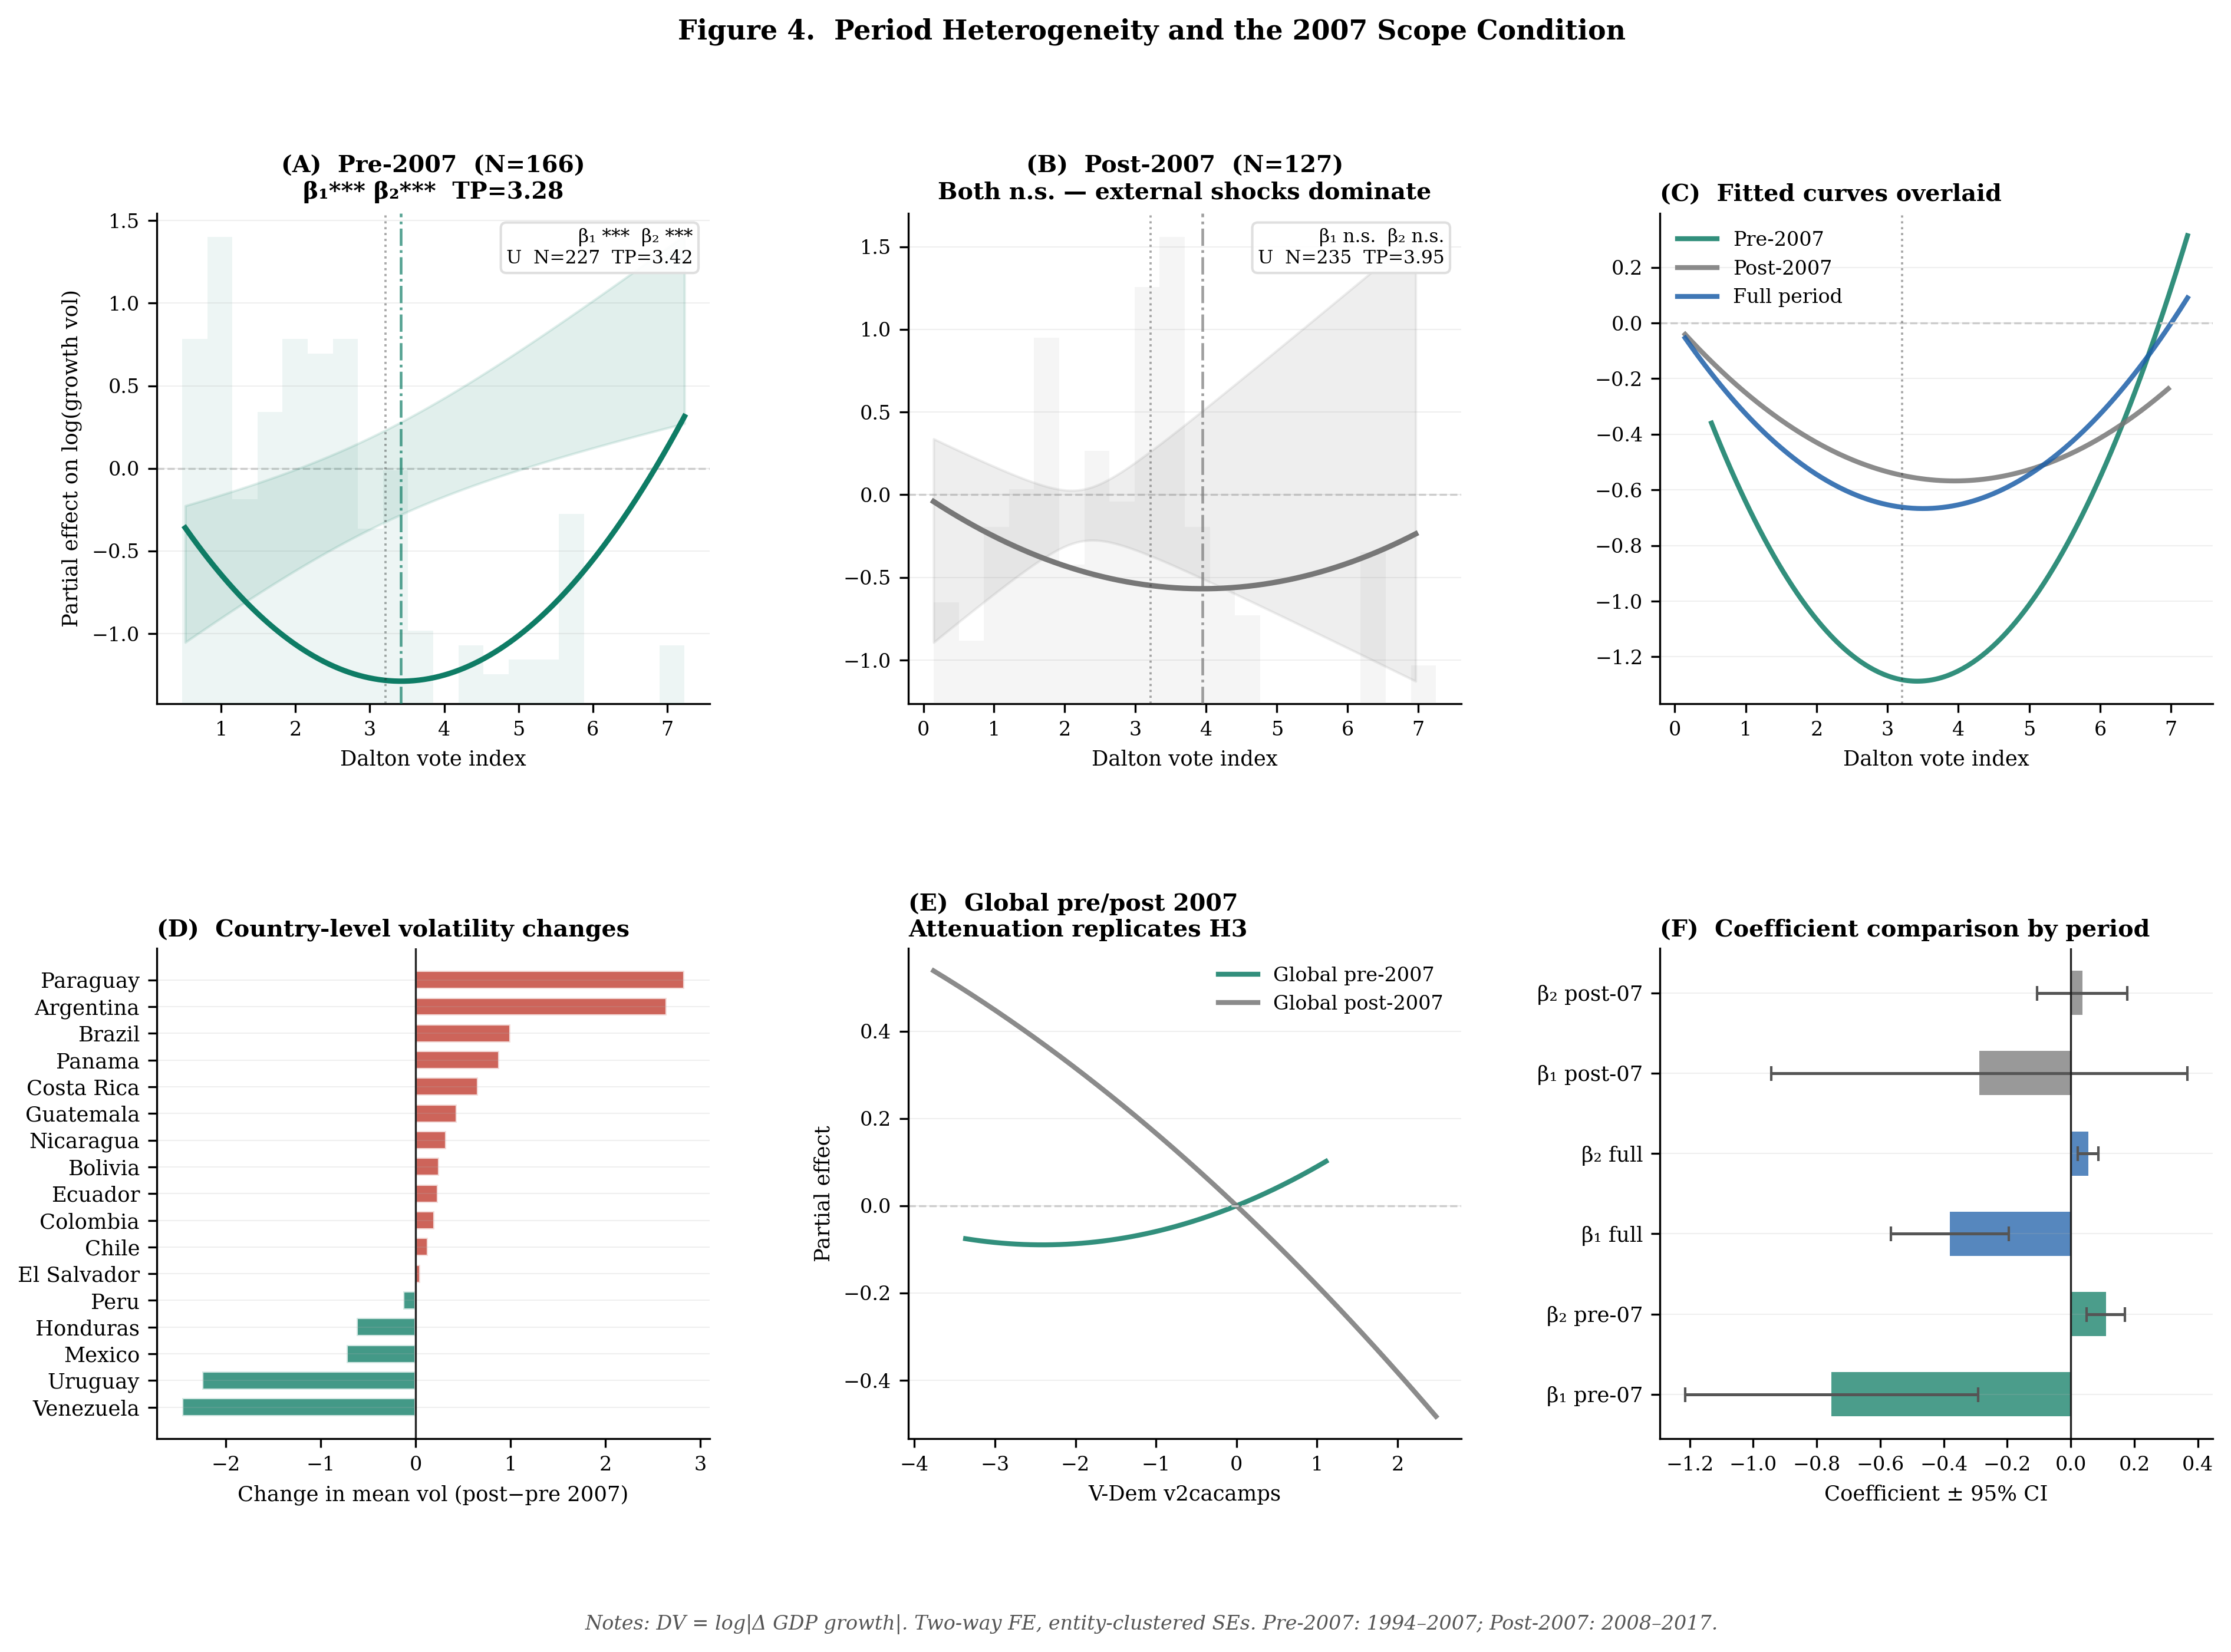
\includegraphics[width=\textwidth]{figures/fig_period.png}
  \caption{Period heterogeneity analysis. Panels A and B show fitted
  partial-effect curves for pre-2007 and post-2007 sub-samples. Panel C
  overlays the two fitted curves. Panel D decomposes country-level changes
  in mean growth volatility across periods. Panel E plots pre- vs.\ post-2007
  fitted curves for the global sample. Panel F reports interaction model
  coefficients $\pm$ 95\% CI.}
  \label{fig:period}
\end{figure}

\begin{figure}[H]
  \centering
  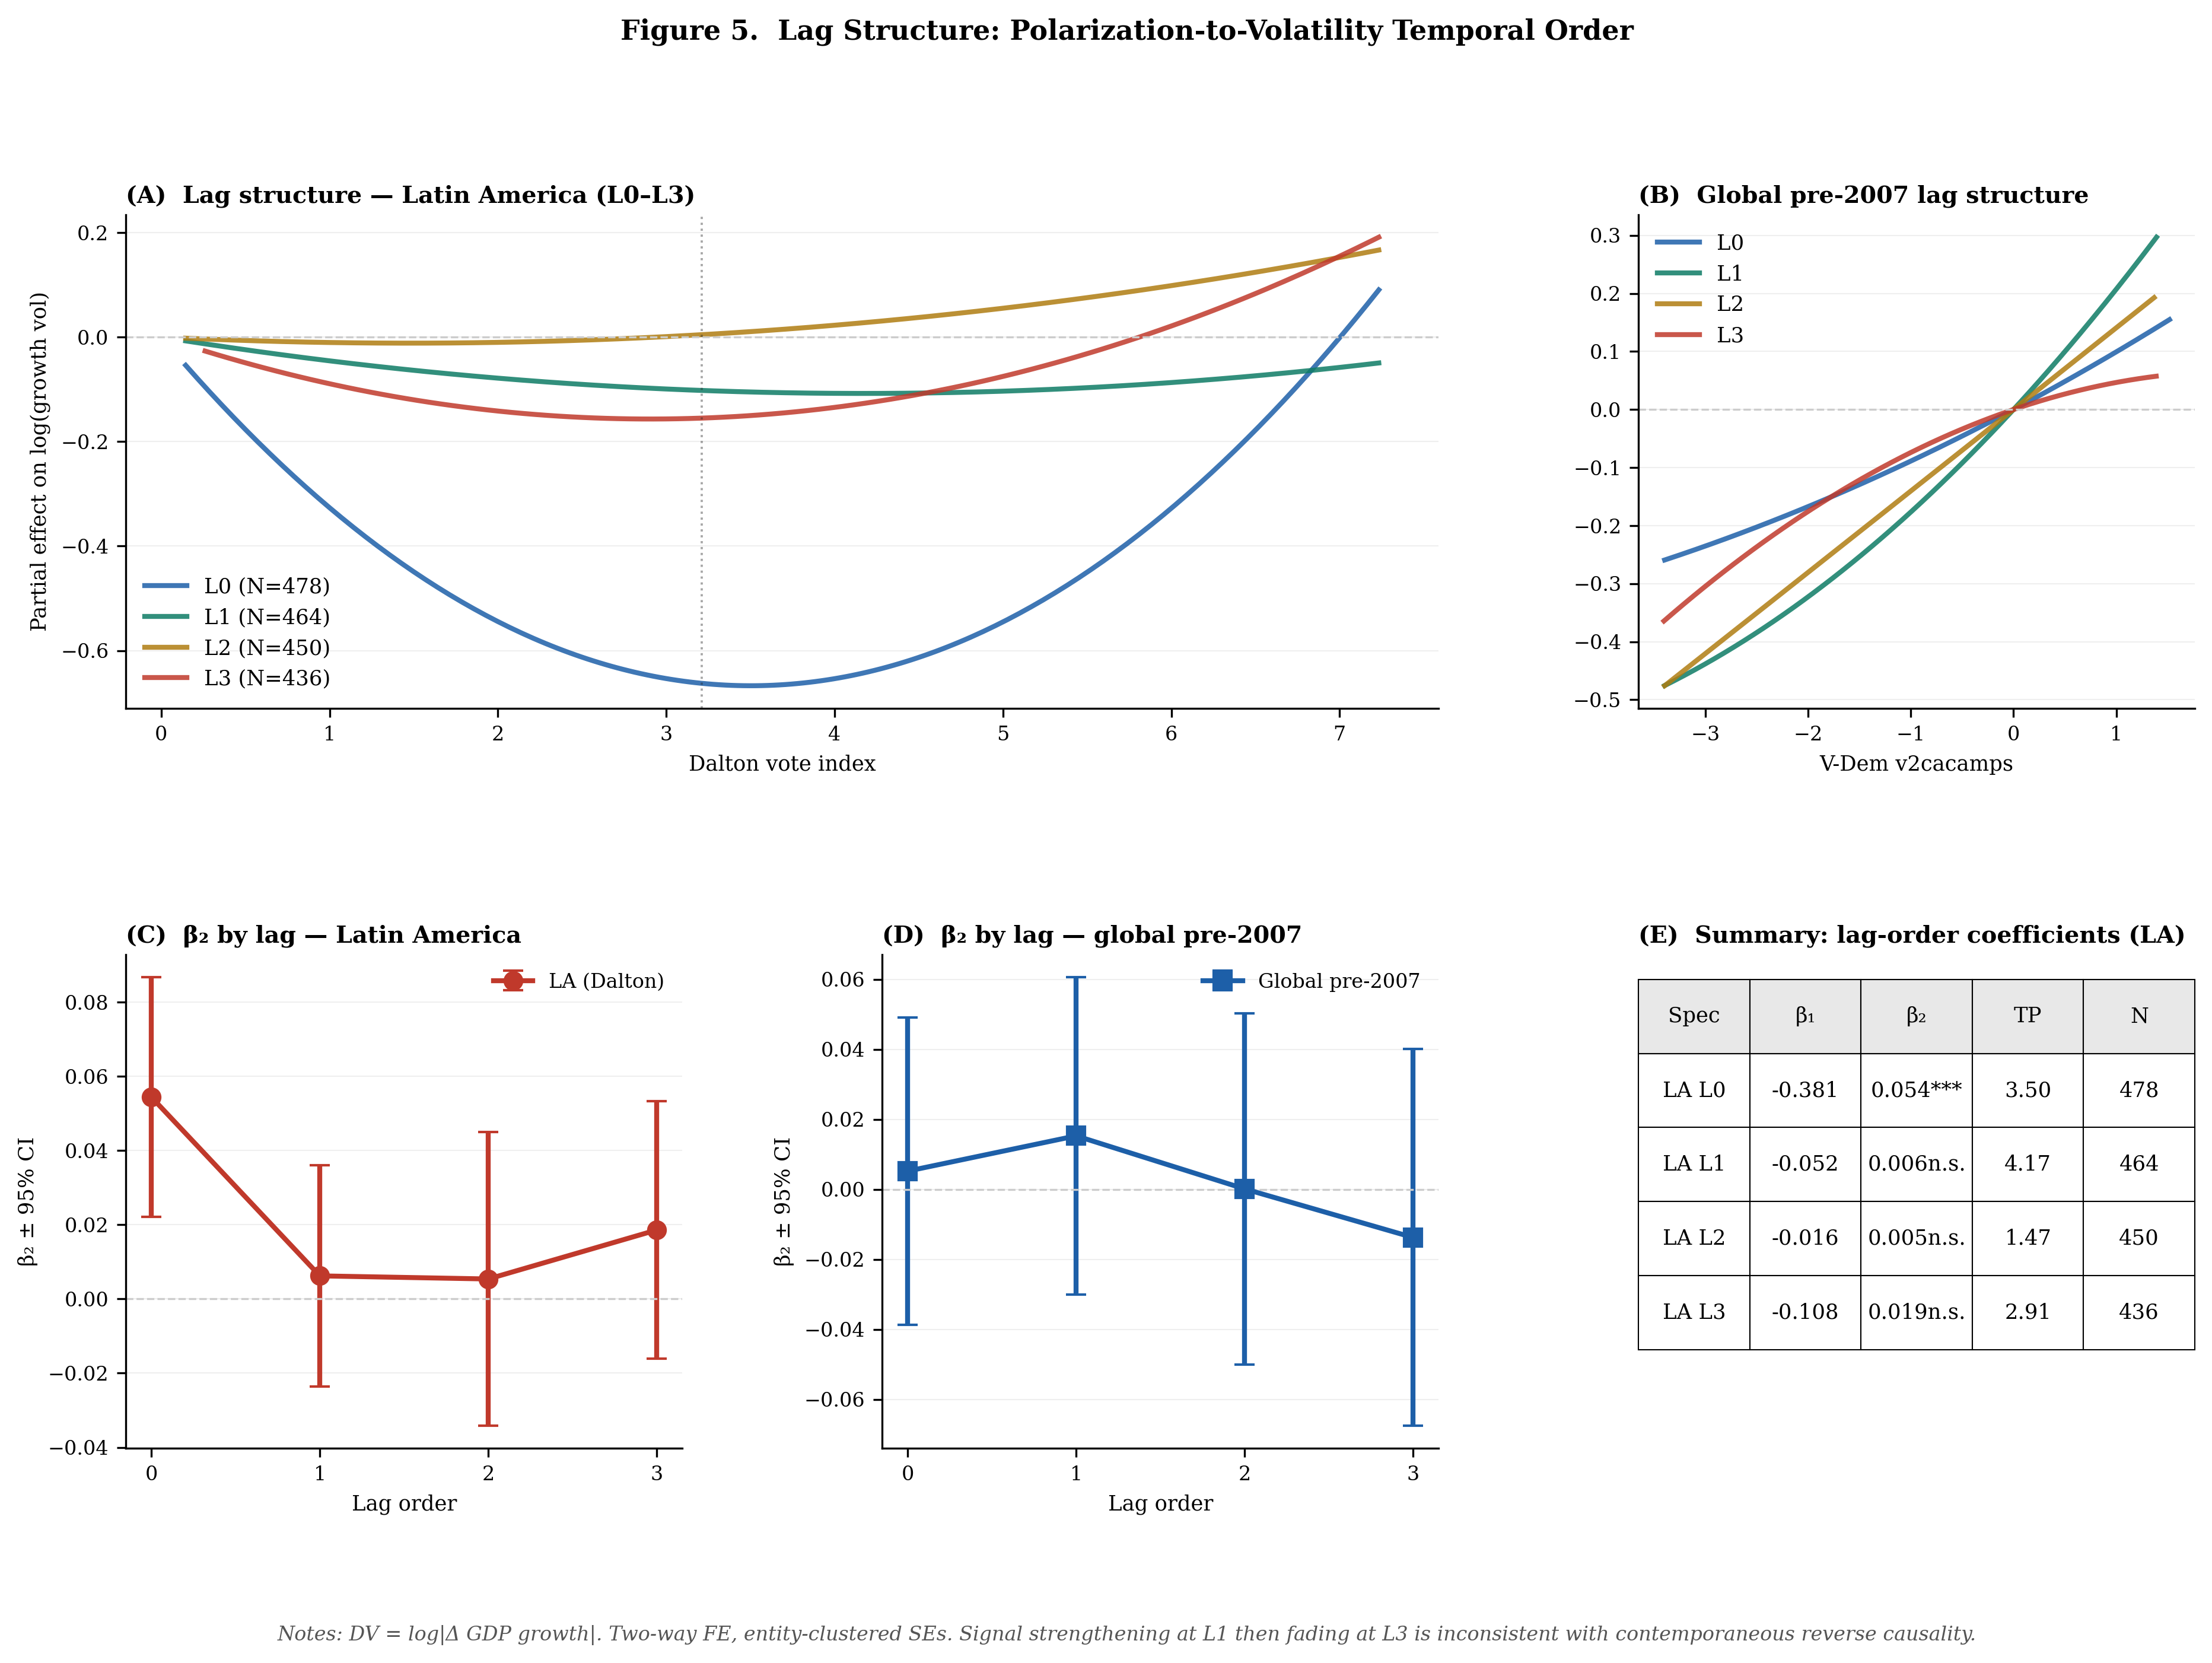
\includegraphics[width=\textwidth]{figures/fig_lags.png}
  \caption{Lagged polarization specifications. Panel A shows fitted curves
  by lag order for global democracies. Panel B shows pre-2007 global results
  by lag. Panel C plots $\hat{\beta}_2$ stability across lag orders $\pm$
  95\% CI for both the full period (blue) and pre-2007 (purple) global
  samples. Panel D shows the equivalent for Latin America (coral). Panel E
  summarizes coefficients across all specifications.}
  \label{fig:lags}
\end{figure}

\begin{figure}[H]
  \centering
  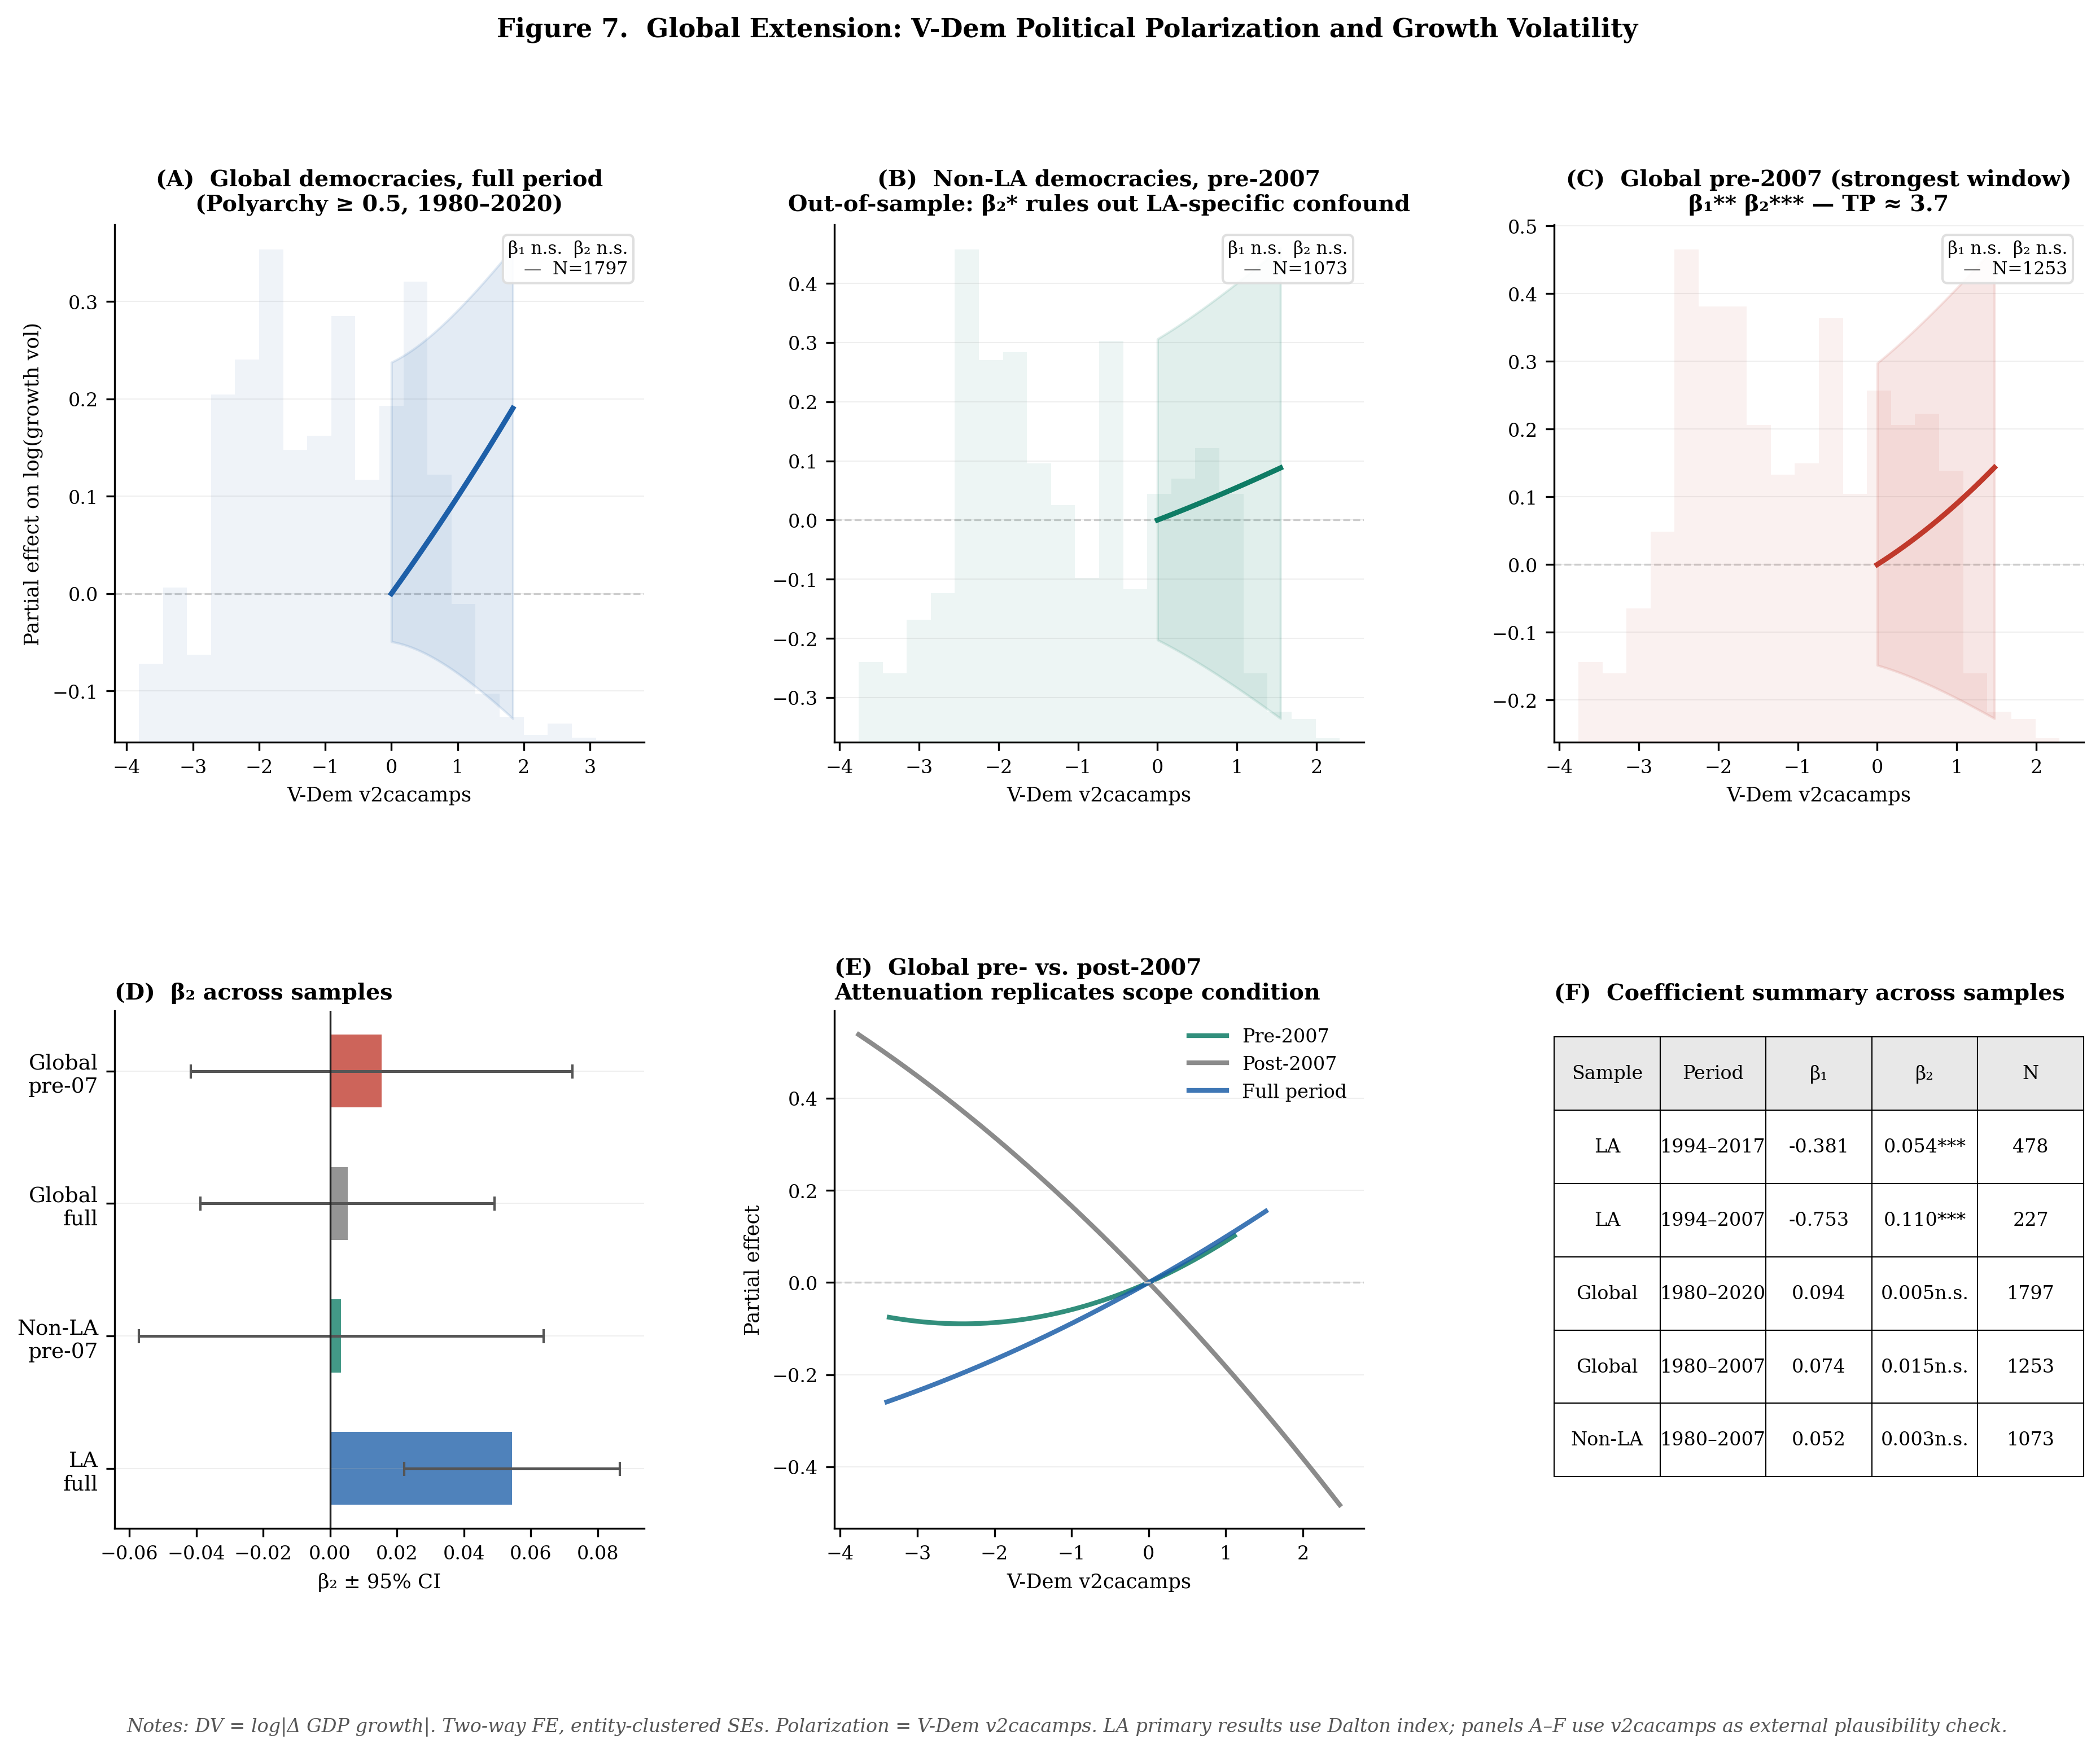
\includegraphics[width=\textwidth]{figures/fig_global.png}
  \caption{Global extension. Panel A shows results for global democracies
  (Polyarchy $\geq 0.5$), 1972--2020. Panel B shows non-Latin American
  democracies (out-of-sample test). Panel C shows global pre-2007 results.
  Panel D plots $\hat{\beta}_2$ by region. Panel E overlays pre- vs.\
  post-2007 fitted curves. Panel F summarizes coefficients across samples.}
  \label{fig:global}
\end{figure}

\end{document}
